%%%%%%%%%%%%%%%%%%%%%%%%%%%%%%%%%%%%%%%%%%%%%%%%%%%%%%%%%%%%%%%%%%%%%%%%%%%%%
%
% Package pgfplots.sty documentation. 
%
% Copyright 2007/2008 by Christian Feuersaenger.
%
% This program is free software: you can redistribute it and/or modify
% it under the terms of the GNU General Public License as published by
% the Free Software Foundation, either version 3 of the License, or
% (at your option) any later version.
% 
% This program is distributed in the hope that it will be useful,
% but WITHOUT ANY WARRANTY; without even the implied warranty of
% MERCHANTABILITY or FITNESS FOR A PARTICULAR PURPOSE.  See the
% GNU General Public License for more details.
% 
% You should have received a copy of the GNU General Public License
% along with this program.  If not, see <http://www.gnu.org/licenses/>.
%
%
%%%%%%%%%%%%%%%%%%%%%%%%%%%%%%%%%%%%%%%%%%%%%%%%%%%%%%%%%%%%%%%%%%%%%%%%%%%%%
\pdfminorversion=5 % to allow compression
\pdfobjcompresslevel=2
\documentclass[a4paper]{ltxdoc}

\usepackage{makeidx}

% DON't let hyperref overload the format of index and glossary. 
% I want to do that on my own in the stylefiles for makeindex...
\makeatletter
\let\@old@wrindex=\@wrindex
\makeatother

\usepackage{ifpdf}
\usepackage[pdfborder=0 0 0]{hyperref}
	\hypersetup{%
		colorlinks=true,	% use true to enable colors below:
		linkcolor=blue,%red,
		filecolor=blue,%magenta,
		pagecolor=blue,%red,
		urlcolor=blue,%cyan,
		citecolor=blue,
		%frenchlinks=false,	% small caps instead of colors
		pdfborder=0 0 0,	% PDF link-darstellung, falls colorlinks=false. 0 0 0: nix. 0 0 1: default.
		%plainpages=false,	% Das ist notwendig, wenn die Seitenzahlen z.T. in Arabischen und z.T. in römischen Ziffern gemacht werden.
		pdftitle=Package PGFPLOTS manual,
		pdfauthor=Christian Feuersänger,
		%pdfsubject=,
		pdfkeywords={pgfplots pgf tikz tex latex},
	}

\makeatletter
\let\@wrindex=\@old@wrindex
\makeatother


\makeatletter
% disables colorlinks for all following \ref commands
\def\pgfplotsmanualdisablecolorforref{%
	\pgfutil@ifundefined{pgfplotsmanual@oldref}{%
		\let\pgfplotsmanual@oldref=\ref
	}{}%
	\def\ref##1{%
		\begingroup
		\let\Hy@colorlink=\pgfplots@disabled@Hy@colorlink
		\let\Hy@endcolorlink=\pgfplots@disabled@Hy@endcolorlink
		\pgfplotsmanual@oldref{##1}%
		\endgroup
	}%
}%
\def\pgfplots@disabled@Hy@colorlink#1{\begingroup}%
\def\pgfplots@disabled@Hy@endcolorlink{\endgroup}%
\makeatother

% Formatiere Seitennummern im Index:
\newcommand{\indexpageno}[1]{%
	{\bfseries\hyperpage{#1}}%
}


\newcommand{\R}{\mathbb{R}}
\newcommand{\N}{\mathbb{N}}
\newcommand{\Z}{\mathbb{Z}}

\long\def\COMMENTLOWLEVEL#1\ENDCOMMENT{}
\def\ENDCOMMENT{}

\usepackage{textcomp}
\usepackage{booktabs}

\usepackage{calc}
\usepackage[formats]{listings}
%\usepackage{courier} % don't use it - the '^' character can't be copy-pasted in courier

\usepackage{array}
\lstset{%
	basicstyle=\ttfamily,
	language=[LaTeX]tex, % Seems as if \lstset{language=tex} must be invoked BEFORE loading tikz!?
	tabsize=4,
	breaklines=true,
	breakindent=0pt
}

\ifpdf
	\pdfinfo {
		/Author	(Christian Feuersaenger)
	}

\else
%	\def\pgfsysdriver{pgfsys-dvipdfm.def}
\fi
%\def\pgfsysdriver{pgfsys-pdftex.def}
\usepackage{pgfplots}
\usepackage{pgfplotstable}

\ifpdf
	% this allows to disable the clickable lib from command line using
	% \pdflatex '\def\pgfplotsclickabledisabled{1}%%%%%%%%%%%%%%%%%%%%%%%%%%%%%%%%%%%%%%%%%%%%%%%%%%%%%%%%%%%%%%%%%%%%%%%%%%%%%
%
% Package pgfplots.sty documentation. 
%
% Copyright 2007/2008 by Christian Feuersaenger.
%
% This program is free software: you can redistribute it and/or modify
% it under the terms of the GNU General Public License as published by
% the Free Software Foundation, either version 3 of the License, or
% (at your option) any later version.
% 
% This program is distributed in the hope that it will be useful,
% but WITHOUT ANY WARRANTY; without even the implied warranty of
% MERCHANTABILITY or FITNESS FOR A PARTICULAR PURPOSE.  See the
% GNU General Public License for more details.
% 
% You should have received a copy of the GNU General Public License
% along with this program.  If not, see <http://www.gnu.org/licenses/>.
%
%
%%%%%%%%%%%%%%%%%%%%%%%%%%%%%%%%%%%%%%%%%%%%%%%%%%%%%%%%%%%%%%%%%%%%%%%%%%%%%
%%%%%%%%%%%%%%%%%%%%%%%%%%%%%%%%%%%%%%%%%%%%%%%%%%%%%%%%%%%%%%%%%%%%%%%%%%%%%
%
% Package pgfplots.sty documentation. 
%
% Copyright 2007/2008 by Christian Feuersaenger.
%
% This program is free software: you can redistribute it and/or modify
% it under the terms of the GNU General Public License as published by
% the Free Software Foundation, either version 3 of the License, or
% (at your option) any later version.
% 
% This program is distributed in the hope that it will be useful,
% but WITHOUT ANY WARRANTY; without even the implied warranty of
% MERCHANTABILITY or FITNESS FOR A PARTICULAR PURPOSE.  See the
% GNU General Public License for more details.
% 
% You should have received a copy of the GNU General Public License
% along with this program.  If not, see <http://www.gnu.org/licenses/>.
%
%
%%%%%%%%%%%%%%%%%%%%%%%%%%%%%%%%%%%%%%%%%%%%%%%%%%%%%%%%%%%%%%%%%%%%%%%%%%%%%
\pdfminorversion=5 % to allow compression
\pdfobjcompresslevel=2
\documentclass[a4paper]{ltxdoc}

\usepackage{makeidx}

% DON't let hyperref overload the format of index and glossary. 
% I want to do that on my own in the stylefiles for makeindex...
\makeatletter
\let\@old@wrindex=\@wrindex
\makeatother

\usepackage{ifpdf}
\usepackage[pdfborder=0 0 0]{hyperref}
	\hypersetup{%
		colorlinks=true,	% use true to enable colors below:
		linkcolor=blue,%red,
		filecolor=blue,%magenta,
		pagecolor=blue,%red,
		urlcolor=blue,%cyan,
		citecolor=blue,
		%frenchlinks=false,	% small caps instead of colors
		pdfborder=0 0 0,	% PDF link-darstellung, falls colorlinks=false. 0 0 0: nix. 0 0 1: default.
		%plainpages=false,	% Das ist notwendig, wenn die Seitenzahlen z.T. in Arabischen und z.T. in römischen Ziffern gemacht werden.
		pdftitle=Package PGFPLOTS manual,
		pdfauthor=Christian Feuersänger,
		%pdfsubject=,
		pdfkeywords={pgfplots pgf tikz tex latex},
	}

\makeatletter
\let\@wrindex=\@old@wrindex
\makeatother


\makeatletter
% disables colorlinks for all following \ref commands
\def\pgfplotsmanualdisablecolorforref{%
	\pgfutil@ifundefined{pgfplotsmanual@oldref}{%
		\let\pgfplotsmanual@oldref=\ref
	}{}%
	\def\ref##1{%
		\begingroup
		\let\Hy@colorlink=\pgfplots@disabled@Hy@colorlink
		\let\Hy@endcolorlink=\pgfplots@disabled@Hy@endcolorlink
		\pgfplotsmanual@oldref{##1}%
		\endgroup
	}%
}%
\def\pgfplots@disabled@Hy@colorlink#1{\begingroup}%
\def\pgfplots@disabled@Hy@endcolorlink{\endgroup}%
\makeatother

% Formatiere Seitennummern im Index:
\newcommand{\indexpageno}[1]{%
	{\bfseries\hyperpage{#1}}%
}


\newcommand{\R}{\mathbb{R}}
\newcommand{\N}{\mathbb{N}}
\newcommand{\Z}{\mathbb{Z}}

\long\def\COMMENTLOWLEVEL#1\ENDCOMMENT{}
\def\ENDCOMMENT{}

\usepackage{textcomp}
\usepackage{booktabs}

\usepackage{calc}
\usepackage[formats]{listings}
%\usepackage{courier} % don't use it - the '^' character can't be copy-pasted in courier

\usepackage{array}
\lstset{%
	basicstyle=\ttfamily,
	language=[LaTeX]tex, % Seems as if \lstset{language=tex} must be invoked BEFORE loading tikz!?
	tabsize=4,
	breaklines=true,
	breakindent=0pt
}

\ifpdf
	\pdfinfo {
		/Author	(Christian Feuersaenger)
	}

\else
%	\def\pgfsysdriver{pgfsys-dvipdfm.def}
\fi
%\def\pgfsysdriver{pgfsys-pdftex.def}
\usepackage{pgfplots}
\usepackage{pgfplotstable}

\ifpdf
	% this allows to disable the clickable lib from command line using
	% \pdflatex '\def\pgfplotsclickabledisabled{1}%%%%%%%%%%%%%%%%%%%%%%%%%%%%%%%%%%%%%%%%%%%%%%%%%%%%%%%%%%%%%%%%%%%%%%%%%%%%%
%
% Package pgfplots.sty documentation. 
%
% Copyright 2007/2008 by Christian Feuersaenger.
%
% This program is free software: you can redistribute it and/or modify
% it under the terms of the GNU General Public License as published by
% the Free Software Foundation, either version 3 of the License, or
% (at your option) any later version.
% 
% This program is distributed in the hope that it will be useful,
% but WITHOUT ANY WARRANTY; without even the implied warranty of
% MERCHANTABILITY or FITNESS FOR A PARTICULAR PURPOSE.  See the
% GNU General Public License for more details.
% 
% You should have received a copy of the GNU General Public License
% along with this program.  If not, see <http://www.gnu.org/licenses/>.
%
%
%%%%%%%%%%%%%%%%%%%%%%%%%%%%%%%%%%%%%%%%%%%%%%%%%%%%%%%%%%%%%%%%%%%%%%%%%%%%%
\input{pgfplots.preamble.tex}
%\RequirePackage[german,english,francais]{babel}

\pgfplotsmanualexternalexpensivetrue

%\usetikzlibrary{external}
%\tikzexternalize[prefix=figures/]{pgfplots}

\title{%
	Manual for Package \PGFPlots\\
	{\small Version \pgfplotsversion}\\
	{\small\href{http://sourceforge.net/projects/pgfplots}{http://sourceforge.net/projects/pgfplots}}}

%\includeonly{pgfplots.libs}


\begin{document}

\def\plotcoords{%
\addplot coordinates {
(5,8.312e-02)    (17,2.547e-02)   (49,7.407e-03)
(129,2.102e-03)  (321,5.874e-04)  (769,1.623e-04)
(1793,4.442e-05) (4097,1.207e-05) (9217,3.261e-06)
};

\addplot coordinates{
(7,8.472e-02)    (31,3.044e-02)    (111,1.022e-02)
(351,3.303e-03)  (1023,1.039e-03)  (2815,3.196e-04)
(7423,9.658e-05) (18943,2.873e-05) (47103,8.437e-06)
};

\addplot coordinates{
(9,7.881e-02)     (49,3.243e-02)    (209,1.232e-02)
(769,4.454e-03)   (2561,1.551e-03)  (7937,5.236e-04)
(23297,1.723e-04) (65537,5.545e-05) (178177,1.751e-05)
};

\addplot coordinates{
(11,6.887e-02)    (71,3.177e-02)     (351,1.341e-02)
(1471,5.334e-03)  (5503,2.027e-03)   (18943,7.415e-04)
(61183,2.628e-04) (187903,9.063e-05) (553983,3.053e-05)
};

\addplot coordinates{
(13,5.755e-02)     (97,2.925e-02)     (545,1.351e-02)
(2561,5.842e-03)   (10625,2.397e-03)  (40193,9.414e-04)
(141569,3.564e-04) (471041,1.308e-04) 
(1496065,4.670e-05)
};
}%
\maketitle
\begin{abstract}%
\PGFPlots\ draws high--quality function plots in normal or logarithmic scaling with a user-friendly interface directly in \TeX. The user supplies axis labels, legend entries and the plot coordinates for one or more plots and \PGFPlots\ applies axis scaling, computes any logarithms and axis ticks and draws the plots, supporting line plots, scatter plots, piecewise constant plots, bar plots, area plots, mesh-- and surface plots and some more. It is based on Till Tantau's package \PGF/\Tikz.
\end{abstract}
\tableofcontents
\section{Introduction}
This package provides tools to generate plots and labeled axes easily. It draws normal plots, logplots and semi-logplots, in two and three dimensions. Axis ticks, labels, legends (in case of multiple plots) can be added with key-value options. It can cycle through a set of predefined line/marker/color specifications. In summary, its purpose is to simplify the generation of high-quality function and/or data plots, and solving the problems of
\begin{itemize}
	\item consistency of document and font type and font size,
	\item direct use of \TeX\ math mode in axis descriptions,
	\item consistency of data and figures (no third party tool necessary),
	\item inter document consistency using preamble configurations and styles.
\end{itemize}
Although not necessary, separate |.pdf| or |.eps| graphics can be generated using the |external| library developed as part of \Tikz.

\PGFPlots\ is build completely on \Tikz/\PGF. Knowledge of \Tikz\ will simplify the work with \PGFPlots, although it is not required.

\section[About PGFPlots: Preliminaries]{About {\normalfont\PGFPlots}: Preliminaries}
This section contains information about upgrades, the team, the installation (in case you need to do it manually) and troubleshooting. You may skip it completely except for the upgrade remarks.

However, note that this library requires at least \PGF\ version $2.00$. At the time of this writing, many \TeX-distributions still contain the older \PGF\ version $1.18$, so it may be necessary to install a recent \PGF\ prior to using \PGFPlots.

\subsection{Components}
\PGFPlots\ comes with two components:
\begin{enumerate}
	\item the plotting component (which you are currently reading) and
	\item the \PGFPlotstable\ component which simplifies number formatting and postprocessing of numerical tables. It comes as a separate package and has its own manual \href{file:pgfplotstable.pdf}{pgfplotstable.pdf}.
\end{enumerate}

\subsection{Upgrade remarks}
This release provides a lot of improvements which can be found in all detail in \texttt{ChangeLog} for interested readers. However, some attention is useful with respect to the following changes.

\subsubsection{New Optional Features}
\begin{enumerate}
	\item \PGFPlots\ 1.3 comes with user interface improvements. The technical distinction between ``behavior options'' and ``style options'' of older versions is no longer necessary (although still fully supported).

	\item \PGFPlots\ 1.3 has a new feature which allows to \emph{move axis labels tight to tick labels} automatically.

	Since this affects the spacing, it is not enabled be default.

	Use
\begin{codeexample}[code only]
\usepackage{pgfplots}
\pgfplotsset{compat=1.3}
\end{codeexample}
	in your preamble to benefit from the improved spacing\footnote{The |compat=1.3| setting is necessary for new features which move axis labels around like reversed axis. However, \PGFPlots\ will still work as it does in earlier versions, your documents will remain the same if you don't set it explicitly.}.
	Take a look at the next page for the precise definition of |compat|.

	\item \PGFPlots\ 1.3 now supports reversed axes. It is no longer necessary to use work--arounds with negative units.
\pgfkeys{/pdflinks/search key prefixes in/.add={/pgfplots/,}{}}

	Take a look at the |x dir=reverse| key.

	Existing work--arounds will still function properly. Use |\pgfplotsset{compat=1.3}| together with |x dir=reverse| to switch to the new version.
\end{enumerate}

\subsubsection{Old Features Which May Need Attention}
\begin{enumerate}
	\item The |scatter/classes| feature produces proper legends as of version 1.3. This may change the appearance of existing legends of plots with |scatter/classes|.

	\item Due to a small math bug in \PGF\ $2.00$, you \emph{can't} use the math expression `|-x^2|'. It is necessary to use `|0-x^2|' instead. The same holds for
		`|exp(-x^2)|'; use `|exp(0-x^2)|' instead.

		This will be fixed with \PGF\ $>2.00$.

	\item Starting with \PGFPlots\ $1.1$, |\tikzstyle| should \emph{no longer be used} to set \PGFPlots\ options.
	
	Although |\tikzstyle| is still supported for some older \PGFPlots\ options, you should replace any occurance of |\tikzstyle| with |\pgfplotsset{|\meta{style name}|/.style={|\meta{key-value-list}|}}| or the associated |/.append style| variant. See section~\ref{sec:styles} for more detail.
\end{enumerate}
I apologize for any inconvenience caused by these changes.

\begin{pgfplotskey}{compat=\mchoice{1.3,pre 1.3,default,newest} (initially default)}
	The preamble configuration 
\begin{codeexample}[code only]
\usepackage{pgfplots}
\pgfplotsset{compat=1.3}
\end{codeexample}
	allows to choose between backwards compatibility and most recent features.

	\PGFPlots\ version 1.3 comes with new features which may lead to different spacings compared to earlier versions:
	\begin{enumerate}
		\item Version 1.3 comes with the |xlabel near ticks| feature which places (in this case $x$) axis labels ``near'' the tick labels, taking the size of tick labels into account.
		
		Older versions used |xlabel absolute|, i.e.\ an absolute distance between the axis and axis labels (now matter how large or small tick labels are).

		The initial setting \emph{keeps backwards compatibility}.

		You are encouraged to use
\begin{codeexample}[code only]
\usepackage{pgfplots}
\pgfplotsset{compat=1.3}
\end{codeexample}
		in your preamble.
		
		\item Version 1.3 fixes a bug with |anchor=south west| which occurred mainly for reversed axes: the anchors where upside--down. This is fixed now.

		
		If you have written some work--around and want to keep it going, use

		|\pgfplotsset{compat/anchors=pre 1.3}|\pgfmanualpdflabel{/pgfplots/compat/anchors}{} 

		to disable the bug fix.
	\end{enumerate}

	Use |\pgfplotsset{compat=default}| to restore the factory settings.

	The setting |\pgfplotsset{compat=newest}| will always use features of the most recent version. This might result in small changes in the document's appearance.
\end{pgfplotskey}

\subsection{The Team}
\PGFPlots\ has been written mainly by Christian Feuers�nger with many improvements of Pascal Wolkotte and Nick Papior Andersen as a spare time project. We hope it is useful and provides valuable plots.

If you are interested in writing something but don't know how, consider reading the auxiliary manual \href{file:TeX-programming-notes.pdf}{TeX-programming-notes.pdf} which comes with \PGFPlots. It is far from complete, but maybe it is a good starting point (at least for more literature).

\subsection{Acknowledgements}
I thank God for all hours of enjoyed programming. I thank Pascal Wolkotte and Nick Papior Andersen for their programming efforts and contributions as part of the development team. I thank Stefan Tibus, who contributed the |plot shell| feature. I thank Tom Cashman for the contribution of the |reverse legend| feature. Special thanks go to Stefan Pinnow whose tests of \PGFPlots\ lead to numerous quality improvements. Furthermore, I thank Dr.~Schweitzer for many fruitful discussions and Dr.~Meine for his ideas and suggestions. Thanks as well to the many international contributors who provided feature requests or identified bugs or simply manual improvements!

Last but not least, I thank Till Tantau and Mark Wibrow for their excellent graphics (and more) package \PGF\ and \Tikz\ which is the base of \PGFPlots.

\include{pgfplots.install}%
\include{pgfplots.intro}%
\include{pgfplots.reference}%
\include{pgfplots.libs}%
\include{pgfplots.resources}%
\include{pgfplots.importexport}%
\include{pgfplots.basic.reference}%

\printindex

\bibliographystyle{abbrv} %gerapali} %gerabbrv} %gerunsrt.bst} %gerabbrv}% gerplain}
\nocite{pgfplotstable}
\nocite{programmingnotes}
\bibliography{pgfplots}
\end{document}
'
	\expandafter\ifx\csname pgfplotsclickabledisabled\endcsname\relax
		\usepgfplotslibrary{clickable}
	\fi
\fi

%\usepackage{fp}
% ATTENTION:
% this requires pgf version NEWER than 2.00 :
%\usetikzlibrary{fixedpointarithmetic}

\usepgfplotslibrary{dateplot,units,groupplots}

\usepackage[a4paper,left=2.25cm,right=2.25cm,top=2.5cm,bottom=2.5cm,nohead]{geometry}
\usepackage{amsmath,amssymb}
\usepackage{xxcolor}
\usepackage{pifont}
\usepackage[latin1]{inputenc}
\usepackage{amsmath}
\usepackage{eurosym}
\usepackage{nicefrac}

\def\eps{\textsc{eps}}

\input pgfmanual-en-macros.tex


\def\pgfplotsifdocpackageuptodate#1#2{%
	\pgfkeysifdefined{/codeexample/prettyprint/word/.@cmd}{#1}{#2}
}%

\pgfplotsiffileexists{pgfmanual.sty}{%
	\RequirePackage{pgfmanual}
	\pgfplotsifdocpackageuptodate{}{%
		\makeatletter
		\input pgfplotsoldpgfsupp_pgfmanual.code.tex
		\makeatother
	}%
}{%
	\makeatletter
	\input pgfplotsoldpgfsupp_pgfmanual.code.tex
	\makeatother
}%

\makeatletter
\def\pgfplotsmakefilelinkifuseful#1#2{%
	\protect\pgfplotsmakefilelinkifuseful@{#1}{#2}%
}%
\def\pgfplotsmakefilelinkifuseful@#1#2{%
	\edef\temp{#1}%
	\edef\tempb{\jobname}%
	\edef\temp{\meaning\temp}% \meaning normalizes the catcodes.
	\edef\tempb{\meaning\tempb}%
	\ifx\temp\tempb
		% we are processing '#1'. Don't make a link.
		#2%
	\else
		\href{file:#1.pdf}{#2}%
	\fi
}%
\makeatother


\pgfkeys{
	/codeexample/prettyprint/cs arguments/pgfplotscreateplotcyclelist/.initial=2,
	/codeexample/prettyprint/cs/pgfplotscreateplotcyclelist/.code args={#1#2#3}{\pgfmanualpdfref{#1}{#1}\{#2\}\{\pgfmanualprettyprintpgfkeys{#3}\pgfmanualclosebrace},
	/codeexample/prettyprint/cs arguments/tikzset/.initial=1,
	/codeexample/prettyprint/cs/tikzset/.code 2 args={\pgfmanualpdfref{#1}{#1}\{\pgfmanualprettyprintpgfkeys{#2}\pgfmanualclosebrace},
	/codeexample/prettyprint/cs arguments/pgfplotsset/.initial=1,
	/codeexample/prettyprint/cs/pgfplotsset/.code 2 args={\pgfmanualpdfref{#1}{#1}\{\pgfmanualprettyprintpgfkeys{#2}\pgfmanualclosebrace},
	/codeexample/prettyprint/cs arguments/pgfplotstableset/.initial=1,
	/codeexample/prettyprint/cs/pgfplotstableset/.code 2 args={\pgfmanualpdfref{#1}{#1}\{\pgfmanualprettyprintpgfkeys{#2}\pgfmanualclosebrace},
	/codeexample/prettyprint/cs arguments/usepgfplotslibrary/.initial=1,
	/codeexample/prettyprint/cs/usepgfplotslibrary/.code 2 args={\pgfmanualpdfref{#1}{#1}\{\pgfmanualpdfref{#2}{#2}\pgfmanualclosebrace},
	%
	%
	%/codeexample/prettyprint/key value/cycle list/.code 2 args={\pgfmanualprettyprintpgfkeys{#2}},
	/codeexample/prettyprint/key value/xticklabel/.code 2 args={\pgfmanualprettyprintcode{#2}},
	/codeexample/prettyprint/key value/yticklabel/.code 2 args={\pgfmanualprettyprintcode{#2}},
	/codeexample/prettyprint/key value/zticklabel/.code 2 args={\pgfmanualprettyprintcode{#2}},
	/codeexample/prettyprint/key value/includegraphics/.code 2 args={\pgfmanualprettyprintpgfkeys{#2}},
	%
	%
	% whenever an unqualified key is found, the following key prefix
	% list is tried to find a match.
	/pdflinks/search key prefixes in={/pgfplots/table/,/pgfplots/error bars/,/pgfplots/,/pgfplots/plot file/,/tikz/,/pgf/},
	%
	% the link prefix written to the pdf file:
	/pdflinks/internal link prefix=pgfp,
	%
	/pdflinks/warnings=false,
	/pdflinks/codeexample links=true,
	/pdflinks/show labels=false,
}%


% should be used to show something in red which doesn't need to get a
% hyper ref.
%
% Examples are descriptions of key labels.
\def\declaretext#1{\texttt{\declare{#1}}}

% To be used whenever something NEW has been declared.
% In this case, a \pgfmanualpdflabel will be generated using '#1'.
%
% Use '\declaretext' if you only describe something local (for example
% the documentation of key values).
\def\declarelabel#1{%
	\texttt{\declare{#1}}%
	\pgfmanualpdflabel{#1}{}%
}

\def\pgfmanualbar{\char`\|}
\makeatletter

\newif\ifpgfplotsmanualexternalexpensive
\let\pgfplotsmanualexternalexpensivetrue@orig=\pgfplotsmanualexternalexpensivetrue

% use \pgfplotsmanualexternalexpensivetrue to externalize expensive
% examples.
\def\pgfplotsmanualexternalexpensivetrue{%
	\usepgfplotslibrary{external}
	\pgfplotsmanualexternalexpensivetrue@orig
	\tikzexternalize[
		prefix=figures/expensiveexample,
		export=false, % needs to be activated for single pictures (i.e. expensive ones)
		mode=list and make,
		verbose IO=false,
		%xport=true,% FASTER FOR DEBUGGING
	]
		{pgfplots}
	\tikzifexternalizing{%
		\nofiles
		\pgfkeys{/pdflinks/codeexample links=false}%
	}{}%
}%

\newif\ifpgfplots@example@is@expensive

\pgfkeys{
	/codeexample/every codeexample/.append code={%
		\ifpgfplots@example@is@expensive
			\pgfkeys{/tikz/external/export=true}%
			\global\pgfplots@example@is@expensivefalse
		\fi
	}
}

% Write this macro directly in front of \begin{codeexample} (without arguments):
\def\pgfplotsexpensiveexample{%
	\ifpgfplotsmanualexternalexpensive
		\pgfplots@example@is@expensivetrue
	\else
		\message{[NOTE: I am now about to typeset an expensive example. You will need to ENLARGE YOUR TeX MEMORY CAPACITIES if this fails.]}%
	\fi
}%


\newenvironment{addplotoperation}[3][]{
  \begin{pgfmanualentry}
  	{%
	\let\ltxdoc@marg=\marg
	\let\ltxdoc@oarg=\oarg
	\let\ltxdoc@parg=\parg
	\let\ltxdoc@meta=\meta
	\def\marg##1{{\normalfont\ltxdoc@marg{##1}}}%
	\def\oarg##1{{\normalfont\ltxdoc@oarg{##1}}}%
	\def\parg##1{{\normalfont\ltxdoc@parg{##1}}}%
	\def\meta##1{{\normalfont\ltxdoc@meta{##1}}}%
    \pgfmanualentryheadline{\textcolor{gray}{{\ttfamily\char`\\addplot\ }}%
      \declare{\texttt{#2}} \texttt{#3;}}%
	  \unskip
	 \nobreak
    \pgfmanualentryheadline{\textcolor{gray}{\texttt{\char`\\addplot}\oarg{options} }%
      \declare{\texttt{#2}} \texttt{#3} \textcolor{gray}{\meta{trailing path commands}}\texttt{;}}%
	  \unskip
	 \nobreak
    \pgfmanualentryheadline{\textcolor{gray}{{\ttfamily\char`\\addplot3}} $\dotsc$}%
    \def\pgfmanualtest{#1}%
    \ifx\pgfmanualtest\@empty%
      \index{#2@\protect\textcolor{gray}{\protect\texttt{plot}}\protect\texttt{ #2}}%
      \index{Plot operations!plot #2@\protect\texttt{plot #2}}%
    \fi%
	\pgfmanualpdflabel{\textbackslash addplot #2}{}%
	\pgfmanualpdflabel{plot #2}{}%
	\pgfmanualpdflabel{#2}{}%
	}%
    \pgfmanualbody
}
{
  \end{pgfmanualentry}
}

\newenvironment{addplot+}{
  \begin{pgfmanualentry}
  	{%
	\let\ltxdoc@marg=\marg
	\let\ltxdoc@oarg=\oarg
	\let\ltxdoc@parg=\parg
	\let\ltxdoc@meta=\meta
	\def\marg##1{{\normalfont\ltxdoc@marg{##1}}}%
	\def\oarg##1{{\normalfont\ltxdoc@oarg{##1}}}%
	\def\parg##1{{\normalfont\ltxdoc@parg{##1}}}%
	\def\meta##1{{\normalfont\ltxdoc@meta{##1}}}%
    \pgfmanualentryheadline{{\ttfamily\declare{\char`\\addplot+}\oarg{options} \textcolor{gray}{\dots};}}%
    \index{addplot+@\protect\texttt{\protect\textbackslash addplot+}}%
	\pgfmanualpdflabel{\textbackslash addplot+}{}%
	}%
    \pgfmanualbody
}
{
  \end{pgfmanualentry}
}
\newenvironment{addplot3generic}{
  \begin{pgfmanualentry}
  	{%
	\let\ltxdoc@marg=\marg
	\let\ltxdoc@oarg=\oarg
	\let\ltxdoc@parg=\parg
	\let\ltxdoc@meta=\meta
	\def\marg##1{{\normalfont\ltxdoc@marg{##1}}}%
	\def\oarg##1{{\normalfont\ltxdoc@oarg{##1}}}%
	\def\parg##1{{\normalfont\ltxdoc@parg{##1}}}%
	\def\meta##1{{\normalfont\ltxdoc@meta{##1}}}%
    \pgfmanualentryheadline{{\ttfamily\declare{\char`\\addplot3}\oarg{options} \meta{input data} \meta{trailing path commands};}}%
    \index{addplot3@\protect\texttt{\protect\textbackslash addplot3}}%
	\pgfmanualpdflabel{\textbackslash addplot3}{}%
	}%
    \pgfmanualbody
}
{
  \end{pgfmanualentry}
}
\newenvironment{addplot3operation}[3][]{
  \begin{pgfmanualentry}
  	{%
	\let\ltxdoc@marg=\marg
	\let\ltxdoc@oarg=\oarg
	\let\ltxdoc@parg=\parg
	\let\ltxdoc@meta=\meta
	\def\marg##1{{\normalfont\ltxdoc@marg{##1}}}%
	\def\oarg##1{{\normalfont\ltxdoc@oarg{##1}}}%
	\def\parg##1{{\normalfont\ltxdoc@parg{##1}}}%
	\def\meta##1{{\normalfont\ltxdoc@meta{##1}}}%
    \pgfmanualentryheadline{\textcolor{gray}{{\ttfamily\char`\\addplot3\ }}%
      \declare{\texttt{#2}} \texttt{#3;}}%
	  \unskip
	 \nobreak
    \pgfmanualentryheadline{\textcolor{gray}{\texttt{\char`\\addplot3}\oarg{options} }%
      \declare{\texttt{#2}} \texttt{#3} \textcolor{gray}{\meta{trailing path commands}}\texttt{;}}%
    \def\pgfmanualtest{#1}%
    \ifx\pgfmanualtest\@empty%
      \index{#2@\protect\texttt{#2}}%
      \index{Plot operations!addplot3 #2@\protect\texttt{#2}}%
    \fi%
	\pgfmanualpdflabel{\textbackslash addplot3 #2}{}%
	\pgfmanualpdflabel{plot3 #2}{}%
	}%
    \pgfmanualbody
}
{
  \end{pgfmanualentry}
}

\newenvironment{codekey}[1]{%
  \begin{pgfmanualentry}
 	\pgfmanualentryheadline{{\ttfamily\declarekey{#1}\textcolor{gray}{/\pgfmanualpdfref{/handlers/.code}{.code}}=\marg{...}}\hfill}%
	\def\mykey{#1}%
	\def\mypath{}%
	\def\myname{}%
	\firsttimetrue%
	\decompose#1/\nil%
    \pgfmanualbody
}
{
  \end{pgfmanualentry}
}
\newenvironment{codeargskey}[2]{%
  \begin{pgfmanualentry}
  	{\toks0={#2}%
  	\xdef\argpattern{\the\toks0 }%
	}%
  	\pgfmanual@command@to@string\argpattern\argpattern
 	\pgfmanualentryheadline{{\ttfamily\declarekey{#1}\textcolor{gray}{/\pgfmanualpdfref{/handlers/.code}{.code args}}=\texttt{\{\argpattern\}}\marg{...}}\hfill}%
	\def\mykey{#1}%
	\def\mypath{}%
	\def\myname{}%
	\firsttimetrue%
	\decompose#1/\nil%
    \pgfmanualbody
}
{
  \end{pgfmanualentry}
}
\def\pgfmanual@command@to@string#1#2{%
	\expandafter\pgfmanual@command@to@string@@\meaning#1\pgfmanual@EOI{#2}%
}%
\xdef\pgfmanual@glob@TMPa{\meaning\pgfutil@empty}%
\expandafter\def\expandafter\pgfmanual@command@to@string@@\pgfmanual@glob@TMPa#1\pgfmanual@EOI#2{%
	\def#2{#1}%
}%

\newenvironment{pgfplotscodekey}[1]{%
	\begin{codekey}{/pgfplots/#1}%
}
{
  \end{codekey}
}
\newenvironment{pgfplotscodetwokey}[1]{%
  \begin{pgfmanualentry}
 	\pgfmanualentryheadline{{\ttfamily\declarekey{/pgfplots/#1}\textcolor{gray}{/\pgfmanualpdfref{/handlers/.code 2 args}{.code 2 args}}=\marg{...}}\hfill}%
	\def\mykey{/pgfplots/#1}%
	\def\mypath{}%
	\def\myname{}%
	\firsttimetrue%
	\decompose/pgfplots/#1/\nil%
    \pgfmanualbody
}
{
  \end{pgfmanualentry}
}

\newenvironment{pgfplotsxycodekeylist}[1]{%
	\begingroup
	\let\oldpgfmanualentryheadline=\pgfmanualentryheadline
	\def\pgfmanualentryheadline##1{%
		\pgfmanualentryheadline@##1\pgfplots@EOI
	}%
	\def\pgfmanualentryheadline@##1\hfill##2\pgfplots@EOI{%
		\oldpgfmanualentryheadline{{\ttfamily\declarekey{##1}\textcolor{gray}{/\pgfmanualpdfref{/handlers/.code}{.code}}=\marg{...}}\hfill}%
	}
	\begin{pgfplotsxykeylist}{#1}%
}
{
	\end{pgfplotsxykeylist}
	\endgroup
}

\newenvironment{pgfplotskey}[1]{%
  \begin{key}{/pgfplots/#1}%
}
{
  \end{key}
}

\def\choicesep{$\vert$}%
\def\choicearg#1{\texttt{#1}}

\newif\iffirstchoice
\newcommand\mchoice[1]{%
	\begingroup
	\let\margold=\marg
	\def\marg##1{{\normalfont\margold{##1}}}%
	\firstchoicetrue
	\foreach \mchoice@ in {#1} {%
		\iffirstchoice
			\global\firstchoicefalse
		\else
			\choicesep
		\fi
		\choicearg{\mchoice@}%
	}%
	\endgroup
}%




% \begin{xykey}{/path/\x label=value}
% \end{xykey}
%
% has same features with 'default', 'initially' etc as key environment
\newenvironment{xykey}[2][]{%
	\begin{pgfmanualentry}
    \def\extrakeytext{}
	\insertpathifneeded{#2}{#1}%
	\expandafter\pgfutil@in@\expandafter=\expandafter{\mykey}%
	\ifpgfutil@in@%
		\expandafter\xykey@eq\mykey\@nil
	\else
		\expandafter\xykey@noeq\mykey\@nil
	\fi
	\pgfmanualbody
}{%
	\end{pgfmanualentry}
}%

% \begin{xystylekey}{/path/\x label=value}
% \end{xystylekey}
%
% has same features with 'default', 'initially' etc as key environment
\newenvironment{xystylekey}[2][]{%
	\begin{pgfmanualentry}
    \def\extrakeytext{style, }
	\insertpathifneeded{#2}{#1}%
	\expandafter\pgfutil@in@\expandafter=\expandafter{\mykey}%
	\ifpgfutil@in@%
		\expandafter\xykey@eq\mykey\@nil
	\else
		\expandafter\xykey@noeq\mykey\@nil
	\fi
	\pgfmanualbody
}{%
	\end{pgfmanualentry}
}%

% \insertpathifneeded{a key}{/pgfplots} -> assign mykey={/pgfplots/a key}
% \insertpathifneeded{/tikz/a key}{/pgfplots} -> assign mykey={/tikz/a key}
%
% #1: the key
% #2: a default path (or empty)
\def\insertpathifneeded#1#2{%
	\def\insertpathifneeded@@{#2}%
	\ifx\insertpathifneeded@@\empty
		\def\mykey{#1}%
	\else
		\insertpathifneeded@#1\@nil
		\ifpgfutil@in@
			\def\mykey{#1}%
		\else
			\def\mykey{#2/#1}%
		\fi
	\fi
}%
\def\insertpathifneeded@#1#2\@nil{%
	\def\insertpathifneeded@@{#1}%
	\def\insertpathifneeded@@@{/}%
	\ifx\insertpathifneeded@@\insertpathifneeded@@@
		\pgfutil@in@true
	\else
		\pgfutil@in@false
	\fi
}%

% \begin{keylist}[default path]
% 	{/path/option 1=value,/path/option 2=value2}
% \end{keylist}
\newenvironment{keylist}[2][]{%
	\begin{pgfmanualentry}
    \def\extrakeytext{}%
	\foreach \xx in {#2} {%
		\expandafter\insertpathifneeded\expandafter{\xx}{#1}%
		\expandafter\extractkey\mykey\@nil%
	}%
	\pgfmanualbody
}{%
  \end{pgfmanualentry}
}%

\newenvironment{pgfplotskeylist}[1]{%
	\begin{keylist}[/pgfplots]{#1}%
}{%
	\end{keylist}%
}

\newenvironment{anchorlist}[1]{
  \begin{pgfmanualentry}
  	\foreach \xx in {#1} {%
		\pgfmanualentryheadline{Anchor {\ttfamily\declare{\xx}}}%
		\index{\xx @\protect\texttt{\xx} anchor}%
		\index{Anchors!\xx @\protect\texttt{\xx}}
		\expandafter\pgfmanualpdflabel\expandafter{\xx}{}
	}%
    \pgfmanualbody
}
{
  \end{pgfmanualentry}
}

\newenvironment{coordinatesystemlist}[1]{
  \begin{pgfmanualentry}
  	\foreach \xx in {#1} {%
		\pgfmanualentryheadline{Coordinate system {\ttfamily\declare{\xx}}}%
		\index{\xx @\protect\texttt{\xx} coordinate system}%
		\index{Coordinate systems!\xx @\protect\texttt{\xx}}
		\expandafter\pgfmanualpdflabel\expandafter{\xx}{}
	}%
    \pgfmanualbody
}
{
  \end{pgfmanualentry}
}
\renewenvironment{coordinatesystem}[1]{
  \begin{pgfmanualentry}
    \pgfmanualentryheadline{Coordinate system {\ttfamily\declare{#1}}}%
    \index{#1@\protect\texttt{#1} coordinate system}%
    \index{Coordinate systems!#1@\protect\texttt{#1}}
	\pgfmanualpdflabel{#1}{}
    \pgfmanualbody
}
{
  \end{pgfmanualentry}
}

% \begin{xykeylist}[default path]
% 	{/path/option \x1=value,/path/option \x2=value2,/path/option \x3=value}
% \end{xykeylist}
\newenvironment{xykeylist}[2][]{%
	\begin{pgfmanualentry}
    \def\extrakeytext{}
	\foreach \xx in {#2} {%
		\expandafter\insertpathifneeded\expandafter{\xx}{#1}%
		\expandafter\pgfutil@in@\expandafter=\expandafter{\mykey}%
		\ifpgfutil@in@%
			\expandafter\xykey@eq\mykey\@nil
		\else
			\expandafter\xykey@noeq\mykey\@nil
		\fi
	}%
	\pgfmanualbody
}{%
  \end{pgfmanualentry}
}%

\makeatother % FIXME this is almost surely a bug in pgfmanual-en-macros
% \begin{commandlist}
% 	{\command1{arg1},\command2{\arg2}}
% \end{commandlist}
\newenvironment{commandlist}[1]{%
	\begin{pgfmanualentry}
	\foreach \xx in {#1} {%
		\expandafter\extractcommand\xx\@@%
	}%
	\pgfmanualbody
}{%
  \end{pgfmanualentry}
}%

\newenvironment{texif}[1]{%
	\begin{pgfmanualentry}
	\pgfmanualentryheadline{\declare{\texttt{\textbackslash if#1}}\meta{true code}\texttt{\textbackslash else}\meta{else code}\texttt{\textbackslash fi}}%
	\index{if#1}%
	\pgfmanualpdflabel{\\if#1}{}%
	\pgfmanualbody
}{%
  \end{pgfmanualentry}
}%
\makeatletter

\newif\ifxykeyfound

\def\xykey@eq#1=#2\@nil{%
	\def\x{x}%
	\xdef\mykey{#1}%
	\def\xykey@@{#1}%
	\ifx\xykey@@\mykey
		\xykeyfoundfalse
	\else
		\xykeyfoundtrue
	\fi
    \expandafter\extractkey\mykey=#2\@nil%
	\ifxykeyfound
		\def\x{y}%
		\xdef\mykey{#1}%
		\expandafter\extractkey\mykey=#2\@nil%
		\def\x{z}%
		\xdef\mykey{#1}%
		\expandafter\extractkey\mykey=#2\@nil%
	\fi
}
\def\xykey@noeq#1\@nil{%
	\def\x{x}%
	\xdef\mykey{#1}%
	\def\xykey@@{#1}%
	\ifx\xykey@@\mykey
		\xykeyfoundfalse
	\else
		\xykeyfoundtrue
	\fi
    \expandafter\extractkey\mykey\@nil%
	\ifxykeyfound
		\def\x{y}%
		\xdef\mykey{#1}%
		\expandafter\extractkey\mykey\@nil%
		\def\x{z}%
		\xdef\mykey{#1}%
		\expandafter\extractkey\mykey\@nil%
	\fi
}

% \begin{pgfplotsxykey}{\x label=value}
% \end{pgfplotsxykey}
%
% It introduces the path /pgfplots/ automatically.
%
% has same features with 'default', 'initially' etc as key environment
\newenvironment{pgfplotsxykey}[1]{%
	\begin{xykey}[/pgfplots]{#1}%
}{%
	\end{xykey}%
}


\newenvironment{pgfplotsxykeylist}[1]{%
	\begin{xykeylist}[/pgfplots]{#1}%
}{%
	\end{xykeylist}%
}


% the first, optional argument is the default key path to insert.
\newenvironment{plottype}[2][/tikz]{%
	\begin{keylist}[#1]{#2}%
	\end{keylist}
  \begin{pgfmanualentry}
    \pgfmanualentryheadline{\textcolor{gray}{{\ttfamily\char`\\addplot+[\declare{#2}]}}}%
    \pgfmanualbody
}
{
  \end{pgfmanualentry}
}

\def\index@prologue{\section*{Index}\addcontentsline{toc}{section}{Index}
}

\newenvironment{pgfplotstablecolumnkey}{%
  \begin{pgfmanualentry}
 	\pgfmanualentryheadline{{\ttfamily\textcolor{gray}{/pgfplots/table/}\declare{columns/\meta{column name}}\textcolor{gray}{/.style}=\marg{key-value-list}}\hfill}%
	\pgfplotsmanualkeyindex{/pgfplots/table/columns}%
    \pgfmanualbody
}
{
  \end{pgfmanualentry}
}
\newenvironment{pgfplotstabledisplaycolumnkey}{%
  \begin{pgfmanualentry}
 	\pgfmanualentryheadline{{\ttfamily\textcolor{gray}{/pgfplots/table/}\declare{display columns/\meta{index}}\textcolor{gray}{/.style}=\marg{key-value-list}}\hfill}%
	\pgfplotsmanualkeyindex{/pgfplots/table/display columns}%
    \pgfmanualbody
}
{
  \end{pgfmanualentry}
}
\newenvironment{pgfplotstablealiaskey}{%
  \begin{pgfmanualentry}
 	\pgfmanualentryheadline{{\ttfamily\textcolor{gray}{/pgfplots/table/}\declare{alias/\meta{col name}}\textcolor{gray}{/.initial}=\marg{real col name}}\hfill}%
	\pgfplotsmanualkeyindex{/pgfplots/table/alias}%
    \pgfmanualbody
}
{
  \end{pgfmanualentry}
}


\def\pgfplotsmanualkeyindex#1{%
	\def\mypath{#1}%
	\def\myname{}%
	\firsttimetrue%
	\decompose#1/\nil%
}
\newenvironment{pgfplotstablecreateonusekey}{%
  \begin{pgfmanualentry}
 	\pgfmanualentryheadline{{\ttfamily\textcolor{gray}{/pgfplots/table/}\declare{create on use/\meta{col name}}\textcolor{gray}{/.style}=\marg{create options}}\hfill}%
	\def\mykey{/pgfplots/table/create on use}%
    \pgfmanualbody
	\pgfplotsmanualkeyindex{/pgfplots/table/create on use}%
}
{
  \end{pgfmanualentry}
}

\def\pgfplotsassertcmdkeyexists#1{%
	\pgfkeysifdefined{/pgfplots/#1/.@cmd}\relax{%
		\pgfplots@error{DOCUMENTATION ERROR: command key /pgfplots/#1 does not exist!}%
	}%
}%

{
\catcode`\ =12%
\gdef\makespaceexpandable{\def\ { }}}%

\def\pgfplotsassertXYcmdkeyexists#1{%
	{\makespaceexpandable\def\x{x}\edef\pgfplotsassertXYcmdkeyexists@tmp{#1}%
	\pgfkeysifdefined{/pgfplots/\pgfplotsassertXYcmdkeyexists@tmp/.@cmd}\relax{%
		\pgfplots@error{DOCUMENTATION ERROR: command key /pgfplots/#1 does not exist!}%
	}}%
	{\makespaceexpandable\def\x{y}\edef\pgfplotsassertXYcmdkeyexists@tmp{#1}%
	\pgfkeysifdefined{/pgfplots/\pgfplotsassertXYcmdkeyexists@tmp/.@cmd}\relax{%
		\pgfplots@error{DOCUMENTATION ERROR: command key /pgfplots/#1 does not exist!}%
	}}%
}%

\def\pgfplotsshortstylekey #1=#2\pgfeov{%
	\pgfplotsassertcmdkeyexists{#1}%
	\pgfplotsassertcmdkeyexists{#2}%
	\begin{pgfplotskey}{#1=\marg{key-value-list}}
		An abbreviation for \texttt{\pgfmanualpdfref{#2}{#2}/\pgfmanualpdfref{/handlers/.append style}{.append style}=}\marg{key-value-list}.
	\end{pgfplotskey}
}
\def\pgfplotsshortxystylekey #1=#2\pgfeov{%
	\pgfplotsassertXYcmdkeyexists{#1}%
	\pgfplotsassertXYcmdkeyexists{#2}%
	\begin{pgfplotsxykey}{#1=\marg{key-value-list}}
		An abbreviation for {\def\x{x}\texttt{\pgfmanualpdfref{#2}{#2}/\pgfmanualpdfref{/handlers/.append style}{.append style}=}}\marg{key-value-list} 
		(or the respective style for $y$, {\def\x{y}\texttt{\pgfmanualpdfref{#2}{#2}/\pgfmanualpdfref{/handlers/.append style}{.append style}=}}).
	\end{pgfplotsxykey}
}
\def\pgfplotsshortstylekeys #1,#2=#3\pgfeov{%
	\pgfplotsassertcmdkeyexists{#1}%
	\pgfplotsassertcmdkeyexists{#2}%
	\pgfplotsassertcmdkeyexists{#3}%
	\begin{pgfplotskeylist}{%
		#1=\marg{key-value-list},
		#2=\marg{key-value-list}}
		Different abbreviations for \texttt{\pgfmanualpdfref{#3}{#3}/\pgfmanualpdfref{/handlers/.append style}{.append style}=}\marg{key-value-list}.
	\end{pgfplotskeylist}
}
\def\pgfplotsshortxystylekeys #1,#2=#3\pgfeov{%
	\pgfplotsassertXYcmdkeyexists{#1}%
	\pgfplotsassertXYcmdkeyexists{#2}%
	\pgfplotsassertXYcmdkeyexists{#3}%
	\begin{pgfplotsxykeylist}{%
		#1=\marg{key-value-list},
		#2=\marg{key-value-list}}
		Different abbreviations for {\def\x{x}\texttt{\pgfmanualpdfref{#3}{#3}/\pgfmanualpdfref{/handlers/.append style}{.append style}=}}\marg{key-value-list}
		(or the respective style for $y$, {\def\x{y}\texttt{\pgfmanualpdfref{#3}{#3}/\pgfmanualpdfref{/handlers/.append style}{.append style}=}}).
	\end{pgfplotsxykeylist}
}


%
% For using the correct form of including libraries in the manual.
% 
\newenvironment{pgfplotslibrary}[1]{%
  \begin{pgfmanualentry}
    \pgfmanualentryheadline{{\ttfamily\char`\\usepgfplotslibrary\char`\{\declare{#1}\char`\}\space\space \char`\%\space\space  \LaTeX\space and plain \TeX}}%
    \index{#1@\protect\texttt{#1} library}%
    \index{Libraries!#1@\protect\texttt{#1}}%
    \pgfmanualentryheadline{{\ttfamily\char`\\usepgfplotslibrary[\declare{#1}]\space \char`\%\space\space Con\TeX t}}%
    \pgfmanualentryheadline{{\ttfamily\char`\\usetikzlibrary\char`\{\declare{pgfplots.#1}\char`\}\space\space \char`\%\space\space \LaTeX\space and plain \TeX}}%
    \pgfmanualentryheadline{{\ttfamily\char`\\usetikzlibrary[\declare{pgfplots.#1}]\space \char`\%\space\space Con\TeX t}}%
	\pgfmanualpdflabel{#1}{}%
    \pgfmanualbody
}
{
  \end{pgfmanualentry}
}


%
% Creates and shows a colormap with specification '#1'.
\def\pgfplotsshowcolormapexample#1{%
	\pgfplotscreatecolormap{tempcolormap}{#1}%
	\pgfplotsshowcolormap{tempcolormap}%
}

% Shows the colormap named '#1'.
\def\pgfplotsshowcolormap#1{%
	\pgfplotscolormapifdefined{#1}{\relax}{%
		\pgfplotsset{colormap/#1}%
	}%
	\pgfplotscolormaptoshadingspec{#1}{8cm}\result
	\def\tempb{\pgfdeclarehorizontalshading{tempshading}{1cm}}%
	\expandafter\tempb\expandafter{\result}%
	\pgfuseshading{tempshading}%
}

\makeatother

\def\decompose/#1/#2\nil{%
  \def\test{#2}%
  \ifx\test\empty%
    % aha.
    \index{#1@\protect\texttt{#1} key}%
	\ifx\mypath\empty
	\else
		\index{\mypath#1@\protect\texttt{#1}}%
	\fi
    \def\myname{#1}%
	%\pgfmanualpdflabel{#1}{}% No, its better to use fully qualified keys and search if necessary!
  \else%
    \iffirsttime
		\begingroup	
			% also make a pdf link anchor with full key path.
			\def\hyperlabelwithoutslash##1/\nil{%
				\pgfmanualpdflabel{##1}{}%
			}%
			\hyperlabelwithoutslash/#1/#2\nil
		\endgroup
%    CF : disabled for /pgfplots/ prefix.
%		\def\mypath{#1@\protect\texttt{/#1/}!}%
%		\firsttimefalse
		\def\pgfplotslocTMPa{pgfplots}%
		\edef\pgfplotslocTMPb{#1}%
		\ifx\pgfplotslocTMPb\pgfplotslocTMPa
			\def\mypath{}%
		\else
			\def\mypath{#1@\protect\texttt{/#1/}!}%
		\fi
		\firsttimefalse
    \else
      \expandafter\def\expandafter\mypath\expandafter{\mypath#1@\protect\texttt{#1/}!}%
    \fi
    \def\firsttime{}
    \decompose/#2\nil%
  \fi%
}
\def\extracthandler#1#2\@nil{%
  \pgfmanualentryheadline{Key handler \meta{key}{\ttfamily/\declare{#1}}#2}%
  \index{\gobble#1@\protect\texttt{#1} handler}%
  \index{Key handlers!#1@\protect\texttt{#1}}
  \pgfmanualpdflabel{/handlers/#1}%
}
\def\extractcommand#1#2\@@{%
  \pgfmanualentryheadline{\declare{\texttt{\string#1}}#2}%
  \removeats{#1}%
  \index{\strippedat @\protect\myprintocmmand{\strippedat}}%
  \pgfmanualpdflabel{\textbackslash\strippedat}{}%
}
\def\extractenvironement#1#2\@@{%
  \pgfmanualentryheadline{{\ttfamily\char`\\begin\char`\{\declare{#1}\char`\}}#2}%
  \pgfmanualentryheadline{{\ttfamily\ \ }\meta{environment contents}}%
  \pgfmanualentryheadline{{\ttfamily\char`\\end\char`\{\declare{#1}\char`\}}}%
  \index{#1@\protect\texttt{#1} environment}%
  \index{Environments!#1@\protect\texttt{#1}}%
  \pgfmanualpdflabel{#1}{}%
}
\renewenvironment{predefinednode}[1]{
  \begin{pgfmanualentry}
    \pgfmanualentryheadline{Predefined node {\ttfamily\declare{#1}}}%
    \index{#1@\protect\texttt{#1} node}%
    \index{Predefined node!#1@\protect\texttt{#1}}
	\pgfmanualpdflabel{#1}{}%
    \pgfmanualbody
}
{
  \end{pgfmanualentry}
}



\usepackage{nicefrac}

\graphicspath{{figures/}}

\def\preambleconfig{width=7cm,compat=1.3}


\expandafter\pgfplotsset\expandafter{\preambleconfig}


\makeatletter
% And now, invoke
% 	/codeexample/typeset listing/.add={% Preamble:\pgfplotsset{\preambleconfig}}{}}
% since listings are VERBATIM, I need to do some low-level things
% here to get the correct \catcodes:
\pgfkeys{/codeexample/typeset listing/.add code={%
		\ifcode@execute
			\pgfutil@in@{axis}{#1}%
			\ifpgfutil@in@
				{\tiny
					\% Preamble: \pgfmanualpdfref{\textbackslash pgfplotsset}{\pgfmanual@pretty@backslash pgfplotsset}%
						\pgfmanual@pretty@lbrace \expandafter\pgfmanualprettyprintpgfkeys\expandafter{\preambleconfig}\pgfmanual@pretty@rbrace
				}%
			\fi
		\fi
	}{},%
	%/codeexample/typeset listing/.show code,
}%
\makeatother

\pgfplotsset{
	%every axis/.append style={width=7cm},
	filter discard warning=false,
}

\pgfqkeys{/codeexample}{%
	every codeexample/.append style={
		width=8cm,
		/pgfplots/legend style={fill=graphicbackground}
	},
	tabsize=4,
}

\usetikzlibrary{backgrounds,patterns}
% Global styles:
\tikzset{
  shape example/.style={
    color=black!30,
    draw,
    fill=yellow!30,
    line width=.5cm,
    inner xsep=2.5cm,
    inner ysep=0.5cm}
}

\newcommand{\FIXME}[1]{\textcolor{red}{(FIXME: #1)}}

% fuer endvironment 'sidewaysfigure' bspw
% \usepackage{rotating}

\newcommand\Tikz{Ti\textit kZ}
\newcommand\PGF{\textsc{pgf}}
\newcommand\PGFPlots{\pgfplotsmakefilelinkifuseful{pgfplots}{\textsc{pgfplots}}}
\newcommand\PGFPlotstable{\pgfplotsmakefilelinkifuseful{pgfplotstable}{\textsc{PgfplotsTable}}}

\makeindex

% Fix overful hboxes automatically:
\tolerance=2000
\emergencystretch=10pt

\tikzset{prefix=gnuplot/pgfplots_} % prefix for 'plot function'

\author{%
	Christian Feuers\"anger\footnote{\url{http://wissrech.ins.uni-bonn.de/people/feuersaenger}}\\%
	Institut f\"ur Numerische Simulation\\
	Universit\"at Bonn, Germany}


%\RequirePackage[german,english,francais]{babel}

\pgfplotsmanualexternalexpensivetrue

%\usetikzlibrary{external}
%\tikzexternalize[prefix=figures/]{pgfplots}

\title{%
	Manual for Package \PGFPlots\\
	{\small Version \pgfplotsversion}\\
	{\small\href{http://sourceforge.net/projects/pgfplots}{http://sourceforge.net/projects/pgfplots}}}

%\includeonly{pgfplots.libs}


\begin{document}

\def\plotcoords{%
\addplot coordinates {
(5,8.312e-02)    (17,2.547e-02)   (49,7.407e-03)
(129,2.102e-03)  (321,5.874e-04)  (769,1.623e-04)
(1793,4.442e-05) (4097,1.207e-05) (9217,3.261e-06)
};

\addplot coordinates{
(7,8.472e-02)    (31,3.044e-02)    (111,1.022e-02)
(351,3.303e-03)  (1023,1.039e-03)  (2815,3.196e-04)
(7423,9.658e-05) (18943,2.873e-05) (47103,8.437e-06)
};

\addplot coordinates{
(9,7.881e-02)     (49,3.243e-02)    (209,1.232e-02)
(769,4.454e-03)   (2561,1.551e-03)  (7937,5.236e-04)
(23297,1.723e-04) (65537,5.545e-05) (178177,1.751e-05)
};

\addplot coordinates{
(11,6.887e-02)    (71,3.177e-02)     (351,1.341e-02)
(1471,5.334e-03)  (5503,2.027e-03)   (18943,7.415e-04)
(61183,2.628e-04) (187903,9.063e-05) (553983,3.053e-05)
};

\addplot coordinates{
(13,5.755e-02)     (97,2.925e-02)     (545,1.351e-02)
(2561,5.842e-03)   (10625,2.397e-03)  (40193,9.414e-04)
(141569,3.564e-04) (471041,1.308e-04) 
(1496065,4.670e-05)
};
}%
\maketitle
\begin{abstract}%
\PGFPlots\ draws high--quality function plots in normal or logarithmic scaling with a user-friendly interface directly in \TeX. The user supplies axis labels, legend entries and the plot coordinates for one or more plots and \PGFPlots\ applies axis scaling, computes any logarithms and axis ticks and draws the plots, supporting line plots, scatter plots, piecewise constant plots, bar plots, area plots, mesh-- and surface plots and some more. It is based on Till Tantau's package \PGF/\Tikz.
\end{abstract}
\tableofcontents
\section{Introduction}
This package provides tools to generate plots and labeled axes easily. It draws normal plots, logplots and semi-logplots, in two and three dimensions. Axis ticks, labels, legends (in case of multiple plots) can be added with key-value options. It can cycle through a set of predefined line/marker/color specifications. In summary, its purpose is to simplify the generation of high-quality function and/or data plots, and solving the problems of
\begin{itemize}
	\item consistency of document and font type and font size,
	\item direct use of \TeX\ math mode in axis descriptions,
	\item consistency of data and figures (no third party tool necessary),
	\item inter document consistency using preamble configurations and styles.
\end{itemize}
Although not necessary, separate |.pdf| or |.eps| graphics can be generated using the |external| library developed as part of \Tikz.

\PGFPlots\ is build completely on \Tikz/\PGF. Knowledge of \Tikz\ will simplify the work with \PGFPlots, although it is not required.

\section[About PGFPlots: Preliminaries]{About {\normalfont\PGFPlots}: Preliminaries}
This section contains information about upgrades, the team, the installation (in case you need to do it manually) and troubleshooting. You may skip it completely except for the upgrade remarks.

However, note that this library requires at least \PGF\ version $2.00$. At the time of this writing, many \TeX-distributions still contain the older \PGF\ version $1.18$, so it may be necessary to install a recent \PGF\ prior to using \PGFPlots.

\subsection{Components}
\PGFPlots\ comes with two components:
\begin{enumerate}
	\item the plotting component (which you are currently reading) and
	\item the \PGFPlotstable\ component which simplifies number formatting and postprocessing of numerical tables. It comes as a separate package and has its own manual \href{file:pgfplotstable.pdf}{pgfplotstable.pdf}.
\end{enumerate}

\subsection{Upgrade remarks}
This release provides a lot of improvements which can be found in all detail in \texttt{ChangeLog} for interested readers. However, some attention is useful with respect to the following changes.

\subsubsection{New Optional Features}
\begin{enumerate}
	\item \PGFPlots\ 1.3 comes with user interface improvements. The technical distinction between ``behavior options'' and ``style options'' of older versions is no longer necessary (although still fully supported).

	\item \PGFPlots\ 1.3 has a new feature which allows to \emph{move axis labels tight to tick labels} automatically.

	Since this affects the spacing, it is not enabled be default.

	Use
\begin{codeexample}[code only]
\usepackage{pgfplots}
\pgfplotsset{compat=1.3}
\end{codeexample}
	in your preamble to benefit from the improved spacing\footnote{The |compat=1.3| setting is necessary for new features which move axis labels around like reversed axis. However, \PGFPlots\ will still work as it does in earlier versions, your documents will remain the same if you don't set it explicitly.}.
	Take a look at the next page for the precise definition of |compat|.

	\item \PGFPlots\ 1.3 now supports reversed axes. It is no longer necessary to use work--arounds with negative units.
\pgfkeys{/pdflinks/search key prefixes in/.add={/pgfplots/,}{}}

	Take a look at the |x dir=reverse| key.

	Existing work--arounds will still function properly. Use |\pgfplotsset{compat=1.3}| together with |x dir=reverse| to switch to the new version.
\end{enumerate}

\subsubsection{Old Features Which May Need Attention}
\begin{enumerate}
	\item The |scatter/classes| feature produces proper legends as of version 1.3. This may change the appearance of existing legends of plots with |scatter/classes|.

	\item Due to a small math bug in \PGF\ $2.00$, you \emph{can't} use the math expression `|-x^2|'. It is necessary to use `|0-x^2|' instead. The same holds for
		`|exp(-x^2)|'; use `|exp(0-x^2)|' instead.

		This will be fixed with \PGF\ $>2.00$.

	\item Starting with \PGFPlots\ $1.1$, |\tikzstyle| should \emph{no longer be used} to set \PGFPlots\ options.
	
	Although |\tikzstyle| is still supported for some older \PGFPlots\ options, you should replace any occurance of |\tikzstyle| with |\pgfplotsset{|\meta{style name}|/.style={|\meta{key-value-list}|}}| or the associated |/.append style| variant. See section~\ref{sec:styles} for more detail.
\end{enumerate}
I apologize for any inconvenience caused by these changes.

\begin{pgfplotskey}{compat=\mchoice{1.3,pre 1.3,default,newest} (initially default)}
	The preamble configuration 
\begin{codeexample}[code only]
\usepackage{pgfplots}
\pgfplotsset{compat=1.3}
\end{codeexample}
	allows to choose between backwards compatibility and most recent features.

	\PGFPlots\ version 1.3 comes with new features which may lead to different spacings compared to earlier versions:
	\begin{enumerate}
		\item Version 1.3 comes with the |xlabel near ticks| feature which places (in this case $x$) axis labels ``near'' the tick labels, taking the size of tick labels into account.
		
		Older versions used |xlabel absolute|, i.e.\ an absolute distance between the axis and axis labels (now matter how large or small tick labels are).

		The initial setting \emph{keeps backwards compatibility}.

		You are encouraged to use
\begin{codeexample}[code only]
\usepackage{pgfplots}
\pgfplotsset{compat=1.3}
\end{codeexample}
		in your preamble.
		
		\item Version 1.3 fixes a bug with |anchor=south west| which occurred mainly for reversed axes: the anchors where upside--down. This is fixed now.

		
		If you have written some work--around and want to keep it going, use

		|\pgfplotsset{compat/anchors=pre 1.3}|\pgfmanualpdflabel{/pgfplots/compat/anchors}{} 

		to disable the bug fix.
	\end{enumerate}

	Use |\pgfplotsset{compat=default}| to restore the factory settings.

	The setting |\pgfplotsset{compat=newest}| will always use features of the most recent version. This might result in small changes in the document's appearance.
\end{pgfplotskey}

\subsection{The Team}
\PGFPlots\ has been written mainly by Christian Feuers�nger with many improvements of Pascal Wolkotte and Nick Papior Andersen as a spare time project. We hope it is useful and provides valuable plots.

If you are interested in writing something but don't know how, consider reading the auxiliary manual \href{file:TeX-programming-notes.pdf}{TeX-programming-notes.pdf} which comes with \PGFPlots. It is far from complete, but maybe it is a good starting point (at least for more literature).

\subsection{Acknowledgements}
I thank God for all hours of enjoyed programming. I thank Pascal Wolkotte and Nick Papior Andersen for their programming efforts and contributions as part of the development team. I thank Stefan Tibus, who contributed the |plot shell| feature. I thank Tom Cashman for the contribution of the |reverse legend| feature. Special thanks go to Stefan Pinnow whose tests of \PGFPlots\ lead to numerous quality improvements. Furthermore, I thank Dr.~Schweitzer for many fruitful discussions and Dr.~Meine for his ideas and suggestions. Thanks as well to the many international contributors who provided feature requests or identified bugs or simply manual improvements!

Last but not least, I thank Till Tantau and Mark Wibrow for their excellent graphics (and more) package \PGF\ and \Tikz\ which is the base of \PGFPlots.

% main=manual.tex

\subsection{Installation and Prerequisites}
\subsubsection{Licensing}
This program is free software: you can redistribute it and/or modify
it under the terms of the GNU General Public License as published by
the Free Software Foundation, either version 3 of the License, or
(at your option) any later version.

This program is distributed in the hope that it will be useful,
but WITHOUT ANY WARRANTY; without even the implied warranty of
MERCHANTABILITY or FITNESS FOR A PARTICULAR PURPOSE.  See the
GNU General Public License for more details.

A copy of the GNU General Public License can be found in the package file
\begin{verbatim}
doc/latex/pgfplots/gpl-3.0.txt
\end{verbatim}
You may also visit~\url{http://www.gnu.org/licenses}.

\subsubsection{Prerequisites}
\PGFPlots\ requires \PGF\ with \textbf{at least version~$2.0$}. It is used with
\begin{verbatim}
\usepackage{pgfplots}
\end{verbatim}
in your preamble (see section~\ref{sec:tex:dialects} for information about how to use it with Con{\TeX}t and plain \TeX).


%\subsubsection{Installation}
There are several ways how to teach \TeX\ where to find the files. Choose the option which fits your needs best.

\subsubsection{Installation in Windows}
Windows users often use Mik\TeX\ which downloads the latest stable package versions automatically. You do not need to install anything manually here. 

However, Mik\TeX\ provides a feature to install packages locally in its own \TeX-Directory-Structure (TDS). This is the preferred way if you like to install newer version than those of Mik\TeX. The basic idea is to unzip \PGFPlots\ in a directory of your choice and configure the Mik\TeX\ Package Manager to use this specific directory with higher priority than its default paths. If you want to do this, start the Mik\TeX\ Settings using ``Start $\gg$ Programs $\gg$ Mik\TeX\ $\gg$ Settings''. There, use the ``Roots'' menu section. It contains the Mik\TeX\ Package directory as initial configuration. Use ``Add'' to select the directory in which the unzipped \PGFPlots\ tree resides. Then, move the newly added path to the list's top using the ``Up'' button. Then press ``Ok''. For Mik\TeX\ 2.8, you may need to uncheck the ``Show Mik\TeX-maintained root directories'' button to see the newly installed path.

Mik\TeX\ complains if the provided directory is not TDS conform (see section~\ref{pgfplots:tds} for details), so you can't provide a wrong directory here. This method does also work for other packages, but some packages may need some directory restructuring before Mik\TeX\ accepts them.

\subsubsection{Installation of Linux Packages}
At the time of this writing, I am unaware of \PGFPlots\ packages for recent stable Linux distributions. For Ubuntu, there are unofficial Ubuntu Package Repositories which can be added to the Ubuntu Package Tools. The idea is: add a simple URL to the Ubuntu Package Tool, run update and the installation takes place automatically. These URLs are maintained as PPA on Ubuntu Servers.

The \PGFPlots\ download area on sourceforge contains recent links about Ubuntu Package Repositories, go to 
\url{http://sourceforge.net/projects/pgfplots/files} 
and download the readme files with recent links.


\subsubsection{Installation in Any Directory - the \texttt{TEXINPUTS} Variable}
You can simply install \PGFPlots\ anywhere on your disc, for example into
\begin{verbatim}
/foo/bar/pgfplots.
\end{verbatim}
Then, you set the \texttt{TEXINPUTS} variable to
\begin{verbatim}
TEXINPUTS=/foo/bar/pgfplots//:
\end{verbatim}
The trailing~`\texttt{:}' tells \TeX\ to check the default search paths after \lstinline!/foo/bar/pgfplots!. The double slash~`\texttt{//}' tells \TeX\ to search all subdirectories.

If the \texttt{TEXINPUTS} variable already contains something, you can append the line above to the existing \texttt{TEXINPUTS} content.

Furthermore, you should set |TEXDOCS| as well,
\begin{verbatim}
TEXDOCS=/foo/bar/pgfplots//:
\end{verbatim}
so that the \TeX-documentation system finds the files |pgfplots.pdf| and |pgfplotstable.pdf| (on some systems, it is then enough to use |texdoc pgfplots|).

Please refer to your operating systems manual for how to set environment variables.

\subsubsection{Installation Into a Local TDS Compliant \texttt{texmf}-Directory}
\label{pgfplots:tds}
\PGFPlots\ comes in a ``\TeX\ Directory Structure'' (TDS) conforming directory structure, so you can simply unpack the files into a directory which is searched by \TeX\ automatically. Such directories are |~/texmf| on Linux systems, for example.

Copy \PGFPlots\ to a local \texttt{texmf} directory like \lstinline!~/texmf!. You need at least the \PGFPlots\ directories |tex/generic/pgfplots| and |tex/latex/pgfplots|. Then, run \lstinline!texhash! (or some equivalent path--updating command specific to your \TeX\ distribution). 

The TDS consists of several sub directories which are searched separately, depending on what has been requested: the sub-directories |doc/latex/|\meta{package} are used for (\LaTeX) documentation, the sub-directories |doc/generic/|\meta{package} for documentation which apply to \LaTeX\ and other \TeX\ dialects (like plain \TeX\ and Con\TeX t which have their own, respective sub-directories) as well.

Similarly, the |tex/latex/|\meta{package} sub-directories are searched whenever \LaTeX\ packages are requested. The |tex/generic/|\meta{package} sub-directories are searched for packages which work for \LaTeX\ \emph{and} other \TeX\ dialects.

Do not forget to run \lstinline!texhash!.

\subsubsection{Installation If Everything Else Fails...}
If \TeX\ still doesn't find your files, you can copy all \lstinline!.sty! and all |.code.tex|-files (perhaps all |.def| files as well) into your current project's working directory. In fact, you need all which is in the |tex/latex/pgfplots| and |tex/generic/pgfplots| sub directories.

Please refer to \url{http://www.ctan.org/installationadvice/} for more information about package installation.



\subsection{Troubleshooting -- Error Messages}
This section discusses some problems which may occur when using \PGFPlots.
Some of the error messages are shown in the index, take a look at the end of this manual (under ``Errors'').


\subsubsection{Problems with available Dimen-registers}
To avoid problems with the many required \TeX-registers for \PGF\ and \PGFPlots, you may want to include
\begin{verbatim}
\usepackage{etex}
\end{verbatim}
as first package. This avoids problems with ``no room for a new dimen''
\index{Error Messages!No room for a new dimen}%
in most cases. It should work with any modern installation of \TeX\ (it activates the e-\TeX\ extensions).

\subsubsection{Dimension Too Large Errors}
The core mathematical engine of \PGF\ relies on \TeX\ registers to perform fast arithmetics. To compute $50+299$, it actually computes |50pt+299pt| and strips the |pt| suffix of the result. Since \TeX\ registers can only contain numbers up to $\pm 16384$, overflow error messages like ``Dimension too large'' occur if the result leaves the allowed range. Normally, this should never happen -- \PGFPlots\ uses a floating point unit with data range $\pm 10^{324}$ and performs all mappings automatically. However, there are some cases where this fails. Some of these cases are:
\begin{enumerate}
	\item The axis range (for example, for $x$) becomes \emph{relatively} small. It's no matter if you have absolutely small ranges like $[10^{-17},10^{-16}]$. But if you have an axis range like $[1.99999999,2]$, where a lot of significant digits are necessary, this may be problematic.
	\item This may happen as well if you only view a very small portion of the data range.
	\item The |axis equal| key will be confused if $x$ and $y$ have a very different scale.
	\item You may have found a bug -- please contact the developers.
\end{enumerate}

\subsubsection{Restrictions for DVI-Viewers and \texttt{dvipdfm}}
\label{sec:drivers}%
\PGF\ is compatible with 
\begin{itemize}
	\item \lstinline!latex!/\lstinline!dvips!,
	\item \lstinline!latex!/\lstinline!dvipdfm!,
	\item \lstinline!pdflatex!,
	\item $\vdots$
\end{itemize}
However, there are some restrictions: I don't know any DVI viewer which is capable of viewing the output of \PGF\ (and therefor \PGFPlots\ as well). After all, DVI has never been designed to draw something different than text and horizontal/vertical lines. You will need to view the postscript file or the pdf-file. 

Then, the DVI/pdf combination doesn't support all types of shadings (for example, the |shader=interp| is only available for |dvips| and |pdftex| drivers).

Furthermore, \PGF\ needs to know a \emph{driver} so that the DVI file can be converted to the desired output. Depending on your system, you need the following options:
\begin{itemize}
	\item \lstinline!latex!/\lstinline!dvips! does not need anything special because \lstinline!dvips! is the default driver if you invoke \lstinline!latex!.
	\item \lstinline!pdflatex! will also work directly because \lstinline!pdflatex! will be detected automatically.
	\item \lstinline!latex!/\lstinline!dvipdfm! requires to use
\begin{verbatim}
\def\pgfsysdriver{pgfsys-dvipdfm.def}
%\def\pgfsysdriver{pgfsys-pdftex.def}
%\def\pgfsysdriver{pgfsys-dvips.def}
\usepackage{pgfplots}.
\end{verbatim}
	The uncommented commands could be used to set other drivers explicitly.
\end{itemize}
Please read the corresponding sections in~\cite[Section 7.2.1 and 7.2.2]{tikz} if you have further questions. These sections also contain limitations of particular drivers.

The choice which won't produce any problems at all is |pdflatex|.

\subsubsection{Problems with \TeX's Memory Capacities}
\PGFPlots\ can handle small up to medium sized plots. However, \TeX\ has never been designed for data plots -- you will eventually face the problem of small memory capacities. See section~\ref{sec:pgfplots:optimization} for how to enlarge them.

\subsubsection{Problems with Language Settings and Active Characters}
Both, \PGF\ and \PGFPlots\ use a lot of characters -- which may lead to incompatibilities with other packages which define active characters. Compatibility is better than in earlier versions, but may still be an issue. The manual compiles with the |babel| package for english and french, the |german| package does also work. If you experience any trouble, let me know. Sometimes it may work to disable active characters temporarily (|babel| provides such a command).

\subsubsection{Other Problems}
Please read the mailing list at

\url{http://sourceforge.net/projects/pgfplots/support}.

\noindent Perhaps someone has also encountered your problem before, and maybe he came up with a solution.

Please write a note on the mailing list if you have a different problem. In case it is necessary to contact the authors directly, consider the addresses shown on the title page of this document.
%
% main=pgfplots.tex

\section{User's Guide: Drawing Axes and Plots}
\subsection{\TeX-dialects: \LaTeX, Con{\TeX}t, plain \TeX }
\label{sec:tex:dialects}%
\PGFPlots\ is compatible with \LaTeX, Con{\TeX}t and plain \TeX. The only difference is how to specify environments. This affects any \PGF/\Tikz-environments and all \PGFPlots-environments like axis, semilogxaxis, semilogyaxis and loglogaxis:
\begin{description}
\def\HEAD{%
	\small
	%\lstset{boxpos=b,breaklines=false,aboveskip=3pt,belowskip=3pt}%
	%\hspace{-1cm}%
	\begin{tabular}{*{2}{p{4cm}}}%
}%
\item[\LaTeX:] |\usepackage{pgfplots}| and

{\HEAD
\begin{codeexample}[code only]
\begin{tikzpicture}
\begin{axis}
...
\end{axis}
\end{tikzpicture}
\end{codeexample}
&
\begin{codeexample}[code only]
\begin{tikzpicture}
\begin{semilogxaxis}
...
\end{semilogxaxis}
\end{tikzpicture}
\end{codeexample}
\\
\end{tabular}%
}

\begin{codeexample}[code only]
\documentclass[a4paper]{article}

% for dvipdfm:
%\def\pgfsysdriver{pgfsys-dvipdfm.def}
\usepackage{pgfplots}
\pgfplotsset{compat=1.3}% <-- moves axis labels near ticklabels (respects tick label widths)

\begin{document}
\begin{figure}
	\centering
	\begin{tikzpicture}
		\begin{loglogaxis}[xlabel=Cost,ylabel=Error]
		\addplot coordinates {
			(5,     8.31160034e-02)
			(17,    2.54685628e-02)
			(49,    7.40715288e-03)
			(129,   2.10192154e-03)
			(321,   5.87352989e-04)
			(769,   1.62269942e-04)
			(1793,  4.44248889e-05)
			(4097,  1.20714122e-05)
			(9217,  3.26101452e-06)
		};
		\addplot coordinates {
			(7,     8.47178381e-02)
			(31,    3.04409349e-02)
			(111,   1.02214539e-02)
			(351,   3.30346265e-03)
			(1023,  1.03886535e-03)
			(2815,  3.19646457e-04)
			(7423,  9.65789766e-05)
			(18943, 2.87339125e-05)
			(47103, 8.43749881e-06)
		};
		\legend{Case 1,Case 2}
		\end{loglogaxis}
	\end{tikzpicture}
	\caption{A larger example}
\end{figure}
\end{document}
\end{codeexample}

\item[Con{\TeX}t:] |\usemodule[pgfplots]| and

{\HEAD
\begin{codeexample}[code only]
\starttikzpicture
\startaxis
...
\stopaxis
\stoptikzpicture
\end{codeexample}
&
\begin{codeexample}[code only]
\starttikzpicture
\startsemilogxaxis
...
\stopsemilogxaxis
\stoptikzpicture
\end{codeexample}
\\
\end{tabular}%
}

A complete Con{\TeX}t--example file can be found in
\begin{codeexample}[code only]
doc/context/pgfplots/pgfplotsexample.tex.
\end{codeexample}

\item[plain \TeX:] |\input pgfplots.tex| and

{\HEAD
\begin{codeexample}[code only]
\tikzpicture
\axis
...
\endaxis
\endtikzpicture
\end{codeexample}
&
\begin{codeexample}[code only]
\tikzpicture
\semilogxaxis
...
\endsemilogxaxis
\endtikzpicture
\end{codeexample}
\\
\end{tabular}%
}

A complete plain--\TeX--example file can be found in
\begin{codeexample}[code only]
doc/plain/pgfplots/pgfplotsexample.tex.
\end{codeexample}
\end{description}
The default system drivers for |dvips| and |pdftex| work without any additional work; for |dvipdfm|, the |pgfsysdriver| macro needs to be redefined manually (see also section~\ref{sec:drivers}).


\subsection{A First Plot}
Plotting is done using \lstinline|\begin{axis} ... \addplot ...; \end{axis}|, where |\addplot| is the main interface to perform plotting operations.
\begin{codeexample}[]
\begin{tikzpicture}
	\begin{axis}[
		xlabel=Cost,
		ylabel=Error]
	\addplot[color=red,mark=x] coordinates {
		(2,-2.8559703)
		(3,-3.5301677)
		(4,-4.3050655)
		(5,-5.1413136)
		(6,-6.0322865)
		(7,-6.9675052)
		(8,-7.9377747)
	};
	\end{axis}
\end{tikzpicture}
\end{codeexample}


\begin{codeexample}[]
\begin{tikzpicture}
	\begin{axis}[
		xlabel=$x$,
		ylabel={$f(x) = x^2 - x +4$}
	]
	% use TeX as calculator:
	\addplot {x^2 - x +4};
	\end{axis}
\end{tikzpicture}
\end{codeexample}

\begin{codeexample}[]
\begin{tikzpicture}
	\begin{axis}[
		xlabel=$x$,
		ylabel=$\sin(x)$
	]
	% invoke external gnuplot as
	% calculator:
	\addplot gnuplot[id=sin]{sin(x)};
	\end{axis}
\end{tikzpicture}
\end{codeexample}

The |plot coordinates|, |plot expression| and |plot gnuplot| commands are three of the several supported ways to create plots, see section~\ref{sec:addplot} for more details\footnote{Please note that you need \lstinline{gnuplot} installed to use \lstinline{plot gnuplot}.} and the remaining ones (|plot file|, |plot shell|, |plot table| and |plot graphics|). The options `|xlabel|' and `|ylabel|' define axis descriptions.

\subsection{Two Plots in the Same Axis}
Multiple |\addplot|-commands can be placed into the same axis.
	% generated with this statement:
	%\addplot plot[id=filesuffix_noise,domain=-6:5,samples=10] gnuplot{(-x**5 - 242 + (-300 + 600*rand(0)))};
\begin{codeexample}[leave comments]
\begin{tikzpicture}
	\begin{axis}[
		height=9cm,
		width=9cm,
		grid=major,
	]
		
	\addplot gnuplot[id=filesuffix]{(-x**5 - 242)};
	\addlegendentry{model}

	\addplot coordinates {
		(-4.77778,2027.60977)
		(-3.55556,347.84069)
		(-2.33333,22.58953)
		(-1.11111,-493.50066)
		(0.11111,46.66082)
		(1.33333,-205.56286)
		(2.55556,-341.40638)
		(3.77778,-1169.24780)
		(5.00000,-3269.56775)
	};
	\addlegendentry{estimate}
	\end{axis}
\end{tikzpicture}
\end{codeexample}
A legend entry is generated if there are |\addlegendentry| commands (or one |\legend| command).

\subsection{Logarithmic Plots}
Logarithmic plots show $\log x$ versus $\log y$  (or just one logarithmic axis). \PGFPlots\ normally uses the natural logarithm, i.e. basis $e\approx2.718$ (see the key |log basis x|). Now, the axis description also contains minor ticks and the labels are placed at $10^i$.
\begin{codeexample}[]
\begin{tikzpicture}
\begin{loglogaxis}[xlabel=Cost,ylabel=Gain]
\addplot[color=red,mark=x] coordinates {
	(10,100)
	(20,150)
	(40,225)
	(80,340)
	(160,510)
	(320,765)
	(640,1150)
};
\end{loglogaxis}
\end{tikzpicture}
\end{codeexample}
A common application is to visualise scientific data. This is often provided in the format $1.42\cdot10^4$, usually written as 1.42e+04. Suppose we have a numeric table named |pgfplots.testtable|, containing
\begin{codeexample}[code only,tabsize=6]
Level Cost  Error
1     7     8.471e-02
2     31    3.044e-02
3     111   1.022e-02
4     351   3.303e-03
5     1023  1.038e-03
6     2815  3.196e-04
7     7423  9.657e-05
8     18943 2.873e-05
9     47103 8.437e-06
\end{codeexample}
then we can plot |Cost| versus |Error| using
\begin{codeexample}[]
\begin{tikzpicture}
\begin{loglogaxis}[
	xlabel=Cost,
	ylabel=Error]
\addplot[color=red,mark=x] coordinates {
	(5,    8.31160034e-02)
	(17,   2.54685628e-02)
	(49,   7.40715288e-03)
	(129,  2.10192154e-03)
	(321,  5.87352989e-04)
	(769,  1.62269942e-04)
	(1793, 4.44248889e-05)
	(4097, 1.20714122e-05)
	(9217, 3.26101452e-06)
};

\addplot[color=blue,mark=*] 
	table[x=Cost,y=Error] {pgfplots.testtable};

\legend{Case 1,Case 2}
\end{loglogaxis}
\end{tikzpicture}
\end{codeexample}
The first plot employs inline coordinates; the second one reads numerical data from file and plots column `|Cost|' versus `|Error|'.

\noindent
Besides the environment ``|loglogaxis|'' you can use
\begin{itemize}
	\item |\begin{axis}...\end{axis}| for normal plots,
	\item |\begin{semilogxaxis}...\end{semilogxaxis}| for plots which have a normal~$y$ axis and a logarithmic~$x$ axis,
	\item |\begin{semilogyaxis}...\end{semilogyaxis}| the same with $x$~and~$y$ switched,
	\item |\begin{loglogaxis}...\end{loglogaxis}| for double--logarithmic plots.
\end{itemize}
You can also use
\begin{codeexample}[code only]
\begin{axis}[xmode=normal,ymode=log]
...
\end{axis}
\end{codeexample}
which is the same as |\begin{semilogyaxis}...\end{semilogyaxis}|.
\begin{codeexample}[]
\begin{tikzpicture}
	\begin{semilogyaxis}[
		xlabel=Index,ylabel=Value]

	\addplot[color=blue,mark=*] coordinates {
		(1,8)
		(2,16)
		(3,32)
		(4,64)
		(5,128)
		(6,256)
		(7,512)
	};
	\end{semilogyaxis}%
\end{tikzpicture}%
\end{codeexample}

\subsection{Cycling Line Styles}
You can skip the style arguments for |\addplot[...]| to determine plot specifications from a predefined list:
\label{page:plotcoords:src}%
\pgfmanualpdflabel{\textbackslash plotcoords}{}%
\begin{codeexample}[width=4cm]
\begin{tikzpicture}
\begin{loglogaxis}[
	xlabel={Degrees of freedom},
	ylabel={$L_2$ Error}
]
\addplot coordinates {
	(5,8.312e-02)    (17,2.547e-02)   (49,7.407e-03)
	(129,2.102e-03)  (321,5.874e-04)  (769,1.623e-04)
	(1793,4.442e-05) (4097,1.207e-05) (9217,3.261e-06)
};

\addplot coordinates{
	(7,8.472e-02)    (31,3.044e-02)    (111,1.022e-02)
	(351,3.303e-03)  (1023,1.039e-03)  (2815,3.196e-04)
	(7423,9.658e-05) (18943,2.873e-05) (47103,8.437e-06)
};

\addplot coordinates{
	(9,7.881e-02)     (49,3.243e-02)    (209,1.232e-02)
	(769,4.454e-03)   (2561,1.551e-03)  (7937,5.236e-04)
	(23297,1.723e-04) (65537,5.545e-05) (178177,1.751e-05)
};

\addplot coordinates{
	(11,6.887e-02)    (71,3.177e-02)     (351,1.341e-02)
	(1471,5.334e-03)  (5503,2.027e-03)   (18943,7.415e-04)
	(61183,2.628e-04) (187903,9.063e-05) (553983,3.053e-05)
};

\addplot coordinates{
	(13,5.755e-02)     (97,2.925e-02)     (545,1.351e-02)
	(2561,5.842e-03)   (10625,2.397e-03)  (40193,9.414e-04)
	(141569,3.564e-04) (471041,1.308e-04) (1496065,4.670e-05)
};
\legend{$d=2$,$d=3$,$d=4$,$d=5$,$d=6$}
\end{loglogaxis}
\end{tikzpicture}
\end{codeexample}
\noindent
The |cycle list| can be modified, see the reference below.

\subsection{Scaling Plots}
You can use any of the \Tikz\ options to modify the appearance. For example, the ``|scale|'' transformation takes the picture as such and scales it.

\begin{codeexample}[]
\begin{tikzpicture}[scale=0.5]
	\begin{loglogaxis}[
		xlabel={Degrees of freedom},
		ylabel={$L_2$ Error}
	]
	\plotcoords
	\legend{$d=2$,$d=3$,$d=4$,$d=5$,$d=6$}
	\end{loglogaxis}
\end{tikzpicture}

\begin{tikzpicture}[scale=1.1]
	\begin{loglogaxis}[
		xlabel={Degrees of freedom},
		ylabel={$L_2$ Error}
	]
	\plotcoords
	\legend{$d=2$,$d=3$,$d=4$,$d=5$,$d=6$}
	\end{loglogaxis}
\end{tikzpicture}
\end{codeexample}
However, you can also scale plots by assigning a |width=5cm| and/or |height=3cm| argument. This only affects the distance of point coordinates, no font sizes or axis descriptions:
\begin{codeexample}[]
\begin{tikzpicture}
	\begin{loglogaxis}[
		width=6cm,
		xlabel={Degrees of freedom},
		ylabel={$L_2$ Error}
	]
	\plotcoords
	\legend{$d=2$,$d=3$,$d=4$,$d=5$,$d=6$}
	\end{loglogaxis}
\end{tikzpicture}

\begin{tikzpicture}
	\begin{loglogaxis}[
		width=8cm,
		xlabel={Degrees of freedom},
		ylabel={$L_2$ Error}
	]
	\plotcoords
	\legend{$d=2$,$d=3$,$d=4$,$d=5$,$d=6$}
	\end{loglogaxis}
\end{tikzpicture}
\end{codeexample}

Use the predefined styles |normalsize|, |small|, |footnotesize| to adopt font sizes and ticks automatically.

\endinput
%
% main=manual.tex

\section{The Reference}

\input pgfplots.reference.axis-addplot.tex
\input pgfplots.reference.preliminaryoptions.tex
\input pgfplots.reference.2dplots.tex
\input pgfplots.reference.3dplots.tex
\input pgfplots.reference.markers-meta.tex
\input pgfplots.reference.axisdescription.tex
\input pgfplots.reference.scaling.tex
\input pgfplots.reference.3dconfiguration.tex
\input pgfplots.reference.errorbars.tex
\input pgfplots.reference.numberformatting.tex
\input pgfplots.reference.specifyrange.tex
\input pgfplots.reference.tickoptions.tex
\input pgfplots.reference.gridoptions-axiscoordinates.tex
\input pgfplots.reference.styleoptions.tex
\input pgfplots.reference.alignment.tex
\input pgfplots.reference.closingplots.tex
\input pgfplots.reference.symbolic-transformations.tex
\input pgfplots.reference.coordfiltering.tex
\input pgfplots.reference.linefitting.tex
\input pgfplots.reference.miscellaneous.tex
%
\section{Related Libraries}
This section describes some libraries which come with \PGFPlots, but they are more or less special and need to be activated separately.
\pgfmanualpdflabel{\textbackslash usepgfplotslibrary}{}

\subsection{Dates as Input Coordinates}
\begin{pgfplotslibrary}{dateplot}
	A library which allows to use dates like |2008-01-01| or dates with time like |2008-01-01 11:35| as input coordinates in plots. The library converts dates to numbers and tick labels will be pretty-printed dates (or times).

	This library is documented in section~\ref{pgfplots:sec:symbolic:coords} on page~\pageref{pgfplots:sec:date:coords}.
\end{pgfplotslibrary}

\subsection{Clickable Plots}
\begin{pgfplotslibrary}{clickable}
	A library which generates small popups whenever one clicks into a plot. The popup displays the coordinate under the mouse pointer. Furthermore, the library allows to display slopes if one holds the mouse pressed and drags it to another point in the plot.


	It is completely sufficient to write 
\begin{codeexample}[code only]
\usepgfplotslibrary{clickable}
\end{codeexample}
	\noindent in the document preamble. This will automatically prepare every plot.

	The library works with Acrobat Javascript and \pdf\ forms: every plot becomes a push--button. 

	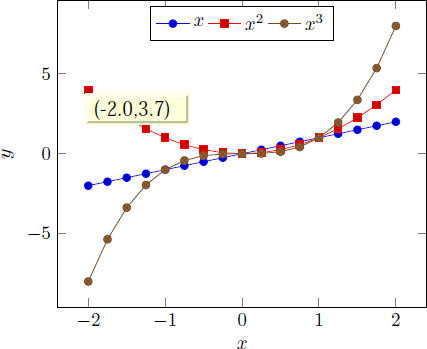
\includegraphics[height=6cm]{figures/pgfplotsclickable-fig1.png}
	\rlap{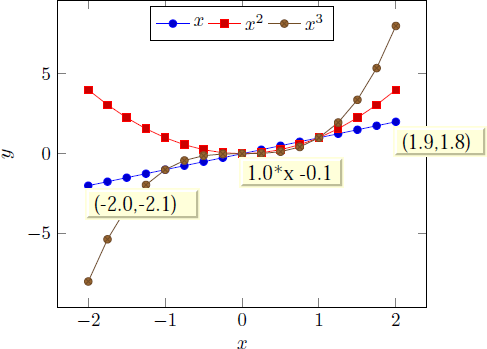
\includegraphics[height=6cm]{figures/pgfplotsclickable-fig2.png}}\hfill

	\nobreak
	These screen shots show the result of clicking into the axis range (left column) and of dragging from one point to another (right column). The second case shows the result of drag- and drop: it displays start- and end points and the equation for the line segment between between the first point of the drag- and drop and the second point where the mouse has been released. The line segment is 
	\[ l(x; x_0,y_0,x_1,y_1) = m \cdot x + n \]
	where $m = (y_1-y_0) / (x_1-x_0)$ is the slope and $n$ the offset chosen such that $l(x_0;\dotsc) = y_0$. For logarithmic plots, logarithms will be applied before computing slopes. 

	\noindent
	\hbox to \linewidth{%
	\hspace{-0.5cm}%
	\begin{tikzpicture}
		\node at (8cm,0cm)	{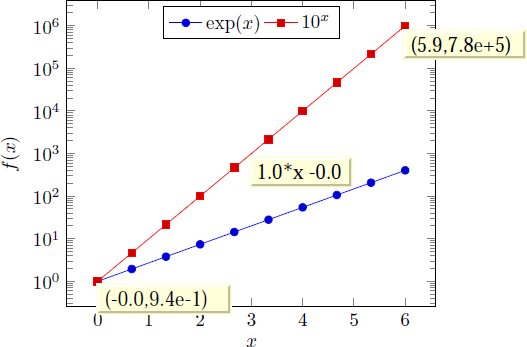
\includegraphics[height=6cm]{figures/pgfplotsclickable-fig4.png}};
		\node at (0cm,0cm)	{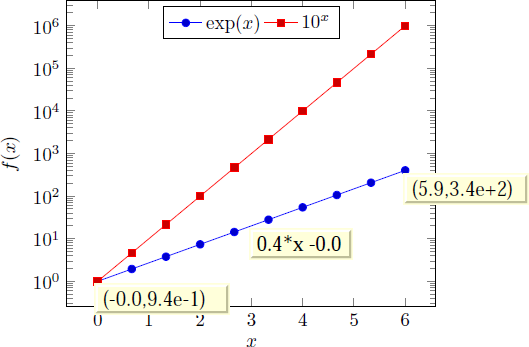
\includegraphics[height=6cm]{figures/pgfplotsclickable-fig3.png}};
	\end{tikzpicture}\hss}%

	\nobreak
	These screen shots show the result of drag- and drop for \emph{logarithmic} axes: the end points show, again, the coordinates (without logs) and the form field in the middle shows the slope and offset of the linear equation in log coordinates.

	The log basis for any logarithmic axes is usually~$10$, but it respects the current setting of |log basis x| and |log basis y|. The applied log will always use the same logarithm which is also used for the axis descriptions (this is not necessarily the same as used by \PGFPlotstable!).

	This document has been produced with the |clickable| library, so it is possible to load it into Acrobat Reader and simply click into a plot.
	
	\expandafter\ifx\csname pgfplotsclickabledisabled\endcsname\relax
	\else
	\paragraph{Attention:} For this document, the |clickable| library has been deactivated. You may find a different version on \url{http://sourceforge.net/projects/pgfplots}.
	\fi

	A click places an annotation at the coordinate under the mouse pointer, a snap--to--nearest feature is not available (yet?).

	\paragraph{Requirements:}
	\begin{itemize}
		\item The library relies on the \LaTeX\ packages |insdljs| (``Insert document level Javascript'') and |eforms| which are both part of the freely available |AcroTeX| education bundle~\cite{acrotex}\footnote{These packages rely on \LaTeX, so the library is only available for \LaTeX, not for plain \TeX\ or Con\TeX t.}. The |insdljs| package creates a temporary file with extension |.djs|.
		
		\item At the time of this writing, only Adobe Acrobat Reader interpretes Javascript and Forms properly. The library doesn't have any effect if the resulting document is used in other viewers (as far as I know).

	\end{itemize}
	Note that although this library has been written for \PGFPlots, it can be used independently of an \PGFPlots\ environment.

	\paragraph{Compatibility issues:}
	There a several restrictions when using this library. Most of them will vanish in future versions -- but up to now, I can't do magic.
	\begin{itemize}
		\item The library does not yet support rotated axes. Use |clickable=false| for those axes.
		\item The library works only with |pdflatex|, |dvips| or |dvipdfm| are not supported\footnote{In fact, they should be. I don't really know why they don't $\hdots$ any hint is welcome.}.

		\item Up to now, it is \emph{not} possible to use this library together with the |external| library and other image externalization methods of section~\ref{sec:pgfplots:importexport}.
		
		To be more precise, you can (with two extra preamble lines, see below) get correctly annotated, exported \pdf\ documents, but the |\includegraphics| command does not import the dynamic features.

		In case you decide to use this work--around, you need to insert
\begin{codeexample}[code only]
% \maxdeadcycles=10000 % in case you get the error `Output loop---<N> consecutive dead cycles.'
\usepackage[pdftex]{eforms}	
\end{codeexample}
		\noindent \emph{before} loading \pgfname, \Tikz\ or \PGFPlots. The |\maxdeadcycles| appears to be necessary for large documents, try it out.

		As long as you are working on a draft version of your document, you might want to use
\begin{codeexample}[code only]
\pgfkeys{/pgf/images/include external/.code={\href{file:#1}{\pgfimage{#1}}}
\end{codeexample}
		in your preamble. This will generate hyper links around the graphics files which link to the exported figures. Clicking on the hyper links opens the exported figure which, in turn, has been generated with the |clickable| library and allows dynamic features\footnote{This special treatment needs the external files in the same base directory as the main document, so this approach is most certainly \emph{not} suitable for a final document.}.


		\item The library automatically calls |\begin{Form}| at |\begin{document}| and |\end{Form}| at the end of the document. This environment of |hyperref| is necessary for dynamic user interaction and should be kept in mind if the document contains other form elements.
	\end{itemize}

	\paragraph{Acknowledgements:}
	\begin{itemize}
		\item I have used a javascript |sprintf| implementation of Kevin van Zonneveld~\cite{phptojs} (the javascript API has only a limited set of conversions).
	\end{itemize}
\end{pgfplotslibrary}

It is possible to customize |pgfplots.clickable| with several options.

\begin{pgfplotskey}{clickable=\mchoice{true,false} (initially true)}
	Allows to disable the library for single plots.
\end{pgfplotskey}

\begin{pgfplotskey}{annot/js fillColor=\marg{javascript color} (initially ["RGB",1,1,.855])}
	Sets the background (fill) color of the short popup annotations. 
	
	Possible choices are |transparent|, gray, RGB or CMYK color specified as four--element--arrays of the form
	|["RGB", |\meta{red}|,|\meta{green}|,|\meta{blue}|]|. Each color component is between $0$ and $1$.

	Again: this option is for Javascript. It is \emph{not} possible to use colors as in \pgfname.
\end{pgfplotskey}

\begin{pgfplotskey}{annot/point format=\marg{sprintf-format} (initially {(\%.1f,\%.1f)})}
	Allows to provide an |sprintf| format string which is used to fill the annotations with text. 
	The first argument to |sprintf| is the $x$-coordinate and the second argument is the $y$-coordinate.

	The |every semilogx axis|, |every semilogy axis| and |every loglog axis| styles have been updated to
\begin{codeexample}[code only]
\pgfplotsset{
	every semilogy axis/.append style={/pgfplots/annot/point format={(\%.1f,\%.1e)}},
	every semilogx axis/.append style={/pgfplots/annot/point format={(\%.1e,\%.1f)}},
	every loglog axis/.append style={/pgfplots/annot/point format={(\%.1e,\%.1e)}}
}
\end{codeexample}
	\noindent such that every logarithmic coordinate is displayed in scientific format.
\end{pgfplotskey}

\begin{pgfplotskey}{annot/slope format=\marg{sprintf-format} (initially \%.1f*x \%+.1f)}
	Allows to provide an |sprintf| format string which is used to fill the slope--annotation with text.
	The first argument is the slope and the second the line offset.
\end{pgfplotskey}

\begin{pgfplotskey}{annot/printable=\mchoice{true,false} (initially false)}
	Allows to configure whether the small annotations will be printed. Otherwise, they are only available on screen.
\end{pgfplotskey}

\begin{pgfplotskey}{annot/font=\marg{javascript font name} (initially font.Times)}
	Allows to choose a javascript font for the annotations. Possible choices are limited to what javascript accepts (which is \emph{not} the same as \LaTeX). The default fonts and its names are shown below.

	\begin{center}
	\begin{tabular}{ll}
		\toprule
		Font Name	& Name in Javascript\\
		\midrule
		Times-Roman           & font.Times\\
        Times-Bold            & font.TimesB\\
        Times-Italic          & font.TimesI\\
        Times-BoldItalic      & font.TimesBI\\
        Helvetica             & font.Helv\\
        Helvetica-Bold        & font.HelvB\\
        Helvetica-Oblique     & font.HelvI\\
        Helvetica-BoldOblique & font.HelvBI\\
        Courier               & font.Cour\\
        Courier-Bold          & font.CourB\\
        Courier-Oblique       & font.CourI\\
        Courier-BoldOblique   & font.CourBI\\
        Symbol                & font.Symbol\\
        ZapfDingbats          & font.ZapfD\\
		\bottomrule
	\end{tabular}
	\end{center}
\end{pgfplotskey}

\begin{pgfplotskey}{annot/textSize=\marg{Size in Point} (initially 11)}
	Sets the text size of annotations in points.
\end{pgfplotskey}

\subsubsection{Using the Clickable Library in Other Contexts}
This library provides essentially one command, |\pgfplotsclickablecreate| which creates a clickable area of predefined size, combined with javascript interaction code. It can be used independently of \PGFPlots.

\begin{command}{\pgfplotsclickablecreate\oarg{required key-value-options}}
	Creates an area which is clickable. A click produces a popup which
	contains information about the point under the cursor.
	
	The complete (!) context needs to be provided using key-value-pairs, either set before
	calling this method of inside of \oarg{required key-value-options}.
	
	This command actually creates an AcroForm which invokes javascript
	whenever it is clicked. A javascript Object is created which
	represents the context (axis limits and options). This javascript
	object is available at runtime.
	
	This method is public and it is \emph{not} restricted to \PGFPlots.
	The \PGFPlots\ hook simply initialises the required key-value-pairs.

	This method does not draw anything. It initialises only a
	clickable area and javascript code.
	
	The required key-value-pairs are documented below.
	
	\paragraph{Attention:} Complete key-value validation is \emph{not} performed here. It
	can happen that invalid options will produce javascript bugs when
	opened with Acrobat Reader. Use the javascript console to find them.
\end{command}

\noindent All options described in the following are only interesting for users who intend to use this library without \PGFPlots.

\begin{pgfplotskey}{annot/width=\marg{dimension} (initially -)}
	This required key communicates the area's width to |\pgfplotsclickablecreate|. It must be a \TeX\ dimension like |5cm|.
\end{pgfplotskey}
\begin{pgfplotskey}{annot/height=\marg{dimension} (initially -)}
	This required key communicates the area's height to |\pgfplotsclickablecreate|. It must be a \TeX\ dimension like |5cm|.
\end{pgfplotskey}
\begin{pgfplotskey}{annot/jsname=\marg{string} (initially -)}
	This required key communicates a unique identifier to |\pgfplotsclickablecreate|. This identifier is used to identify the object in javascript, so there can't be more than one of them. If it is empty, a default identifier will be created.
\end{pgfplotskey}

\begin{pgfplotskeylist}{annot/xmin=\marg{number},annot/xmax=\marg{number},annot/ymin=\marg{number},annot/ymax=\marg{number} (initially empty)}
	These required keys communicate the axis limits to |\pgfplotsclickablecreate|. They should be set to numbers which can be assigned to a javascript floating point number (standard IEEE double precision).
\end{pgfplotskeylist}

\input pgfplots.libs.units.tex
\input pgfplots.libs.groupplot.tex

\subsection{Image Externalization}
\begin{pgfplotslibrary}{external}
	The |external| library offers a convenient method to export every single |tikzpicture| into a separate~|.pdf| (or~|.eps|). Later runs of \LaTeX\ will simply include these graphics, thereby reducing typesetting time considerably.
	
	This library is documented in more detail in section~\ref{sec:pgfplots:export} ``Export to {\pdf/\eps}''.


	The |external| library has been written by Christian Feuers\"anger (author of \PGFPlots). It has been contributed to \Tikz\ as general purpose library, so the reference documentation along with all tweaks can be found in~\cite[Section ``Externalization Library'']{tikz}. The command |\usepgfplotslibrary{external}| is actually just a wrapper which loads |\usetikzlibrary{external}| or, if this library does not yet exist because the installed \pgfname\ has at most version $2.00$, it will load a copy which is shipped with \PGFPlots.
\end{pgfplotslibrary}
%
\section{Memory and Speed considerations}
\subsection{Memory Limits of \TeX}
\label{sec:pgfplots:optimization}
\PGFPlots\ can typeset plots with several thousand points if memory limits of \TeX\ are configured properly. Its runtime is roughly proportional to the number of input points\footnote{In fact, the runtime is pseudo--linear: starting with about $100{,}000$ points, it will become quadratic. This limitation applies to the path length of \PGF\ paths as well. Furthermore, the linear runtime is not possible yet for stacked plots.}.

\pgfplotsexpensiveexample
\begin{codeexample}[]
\begin{tikzpicture}
\begin{axis}[
	enlargelimits=0.01,
	title style={yshift=5pt},
	title=Scatter plot with $2250$ points]
	
\addplot[blue,
	mark=*,only marks,mark options={scale=0.3}]
	file[skip first]
	{plotdata/pgfplots_scatterdata3.dat};
	
\end{axis}
\end{tikzpicture}
\end{codeexample}

\pgfplotsexpensiveexample
\begin{codeexample}[]
\begin{tikzpicture}
\begin{axis}[
	enlarge x limits=0.03,
	title=Ornstein-Uhlenbeck sample
		($13000$ time steps),
	xlabel=$t$]
	
\addplot[blue] file {plotdata/ou.dat};
\end{axis}
\end{tikzpicture}
\end{codeexample}

\pgfplotsexpensiveexample
\begin{codeexample}[]
\begin{tikzpicture}
\begin{axis}[
	title=$120 \times 120$ Smooth Surface,
	xlabel=$x$,
	ylabel=$y$]
\addplot3[surf,samples=120,shader=interp,domain=0:1] 
	{sin(deg(8*pi*x))* exp(-20*(y-0.5)^2) 
	+ exp(-(x-0.5)^2*30 
		- (y-0.25)^2 - (x-0.5)*(y-0.25))};
\end{axis}
\end{tikzpicture}
\end{codeexample}

\PGFPlots\ relies completely on \TeX\ to do all typesetting. It uses the front-end-layer and basic layer of \PGF\ to perform all drawing operations. For complicated plots, this may take some time, and you may want to read section~\ref{sec:pgfplots:importexport} for how to write single figures to external graphics files. Externalization is the best way to reduce typesetting time.

However, for large scale plots with a lot of points, limitations of \TeX's capacities are reached easily.

\subsection{Memory Limitations}
The default settings of most \TeX-distributions are quite restrictive, so it may be necessary to adjust them. 

Usually, the log--file or the final error message contains a summary about the used resources, giving a hint which parameter needs to be increased.

\subsubsection{Mik\TeX}
For Mik\TeX, memory limits can be increased in two ways. The first is to use command line switches:
\begin{codeexample}[code only]
pdflatex 
	--stack-size=n --save-size=n 
	--main-memory=n --extra-mem-top=n --extra-mem-bot=n
	--pool-size=n --max-strings=n 
\end{codeexample}
\noindent Experiment with these settings if Mik\TeX\ runs out of memory. Usually, one doesn't invoke |pdflatex| manually: there is a development aid which does all the invocations, so this one needs to be adjusted. 

Sometimes it might be better to adjust the Mik\TeX\ configuration file permanently, for example to avoid reconfiguring the \TeX\ development program. This can be realized using the command
\begin{codeexample}[code only]
initexmf --edit-config-file=pdflatex
\end{codeexample}
\noindent which can be typed either on a command prompt in Windows or using Start $\gg$ Execute. As a result, an editor will be opened with the correct config file. A sample config file could be
\begin{codeexample}[code only]
main_memory=90000000
save_size=80000
\end{codeexample}
or any of the config file entries which are listed below can be entered. 
Thanks to ``LeSpocky'' for his documentation in

\url{http://blog.antiblau.de/2009/04/21/speicherlimits-von-miktex-erhoehen}.

\subsubsection{\TeX Live or similar installations}
For Unix installations, one needs to adjust config files. This can be done as follows:
\begin{enumerate}
	\item Locate |texmf.cnf| on your system. On my Ubuntu installation, it is in 
	
	|/usr/share/texmf/web2c/texmf.cnf|.
	\item Either change |texmf.cnf| directly, or copy it to some convenient place. If you copy it, here is how to proceed:
		\begin{itemize}
			\item keep only the changed entries in your local copy to reduce conflicts. \TeX\ will always read \emph{all} config files found in its search path.
			\item Adjust the search path to find your local copy. This can be done using the environment variable |TEXMFCNF|. Assuming your local copy is in |~/texmf/mytexcnf/texmf.cnf|, you can write
\begin{codeexample}[code only]
export TEXMFCNF=~/texmf/mytexcnf:
\end{codeexample}
			to search first in your directory, then in all other system directories.
		\end{itemize}
	\item You should change the entries
\begin{codeexample}[code only]
main_memory = n
extra_mem_top = n
extra_mem_bot = n
max_strings = n
param_size = n
save_size = n
stack_size = n
\end{codeexample}
		The log--file usually contains information about the parameter which needs to be enlarged.
\end{enumerate}
An example of this config file thing is shown below. It changes memory limits.
\begin{enumerate}
	\item Create the file |~/texmf/mytexcnf/texmf.cnf| (and possibly the paths as well).
\begin{codeexample}[code only]
% newly created file ~/texmf/mytexcnf/texmf.cnf:
% If you want to change some of these sizes only for a certain TeX
% variant, the usual dot notation works, e.g.,
% main_memory.hugetex = 20000000
main_memory = 230000000 % words of inimemory available; also applies to inimf&mp
extra_mem_top = 10000000     % extra high memory for chars, tokens, etc.
extra_mem_bot = 10000000     % extra low memory for boxes, glue, breakpoints, etc.
save_size = 150000	% for saving values outside current group
stack_size = 150000	% simultaneous input sources

% Max number of characters in all strings, including all error messages,
% help texts, font names, control sequences.  These values apply to TeX and MP.
%pool_size = 1250000
% Minimum pool space after TeX/MP's own strings; must be at least
% 25000 less than pool_size, but doesn't need to be nearly that large.
%string_vacancies = 90000
% Maximum number of strings.
%max_strings = 100000
% min pool space left after loading .fmt
%pool_free = 47500
\end{codeexample}
	\item Run |texhash| such that \TeX\ updates its |~/texmf/ls-R| database.
	\item Create the environment variable |TEXMFCNF| and assign the value `|~/texmf/mytexcnf:|' (including the trailing `|:|'!). For my linux system, this can be done using by adding
\begin{codeexample}[code only]
export TEXMFCNF=~/texmf/mytexcnf:
\end{codeexample}
	to |~/.bashrc|.
\end{enumerate}

Unfortunately, \TeX\ does not allow arbitrary memory limits, there is an upper bound hard coded in the executables.

\subsection{Reducing Typesetting Time}
\PGFPlots\ does a lot of computations ranging from abstract coordinate computations to low level |.pdf| drawing commands (realized by \PGF). For complex plots, this may take a considerable time -- especially for 3D plots.

One possibility to reduce typesetting time is to tell \PGF\ to generate single, temporary |.pdf| (or |.eps|) documents for a subset (or all) graphics in one run and re-use these temporary images in successive runs. For \PGFPlots, this is the most effective way to reduce typesetting time. It can be accomplished using the |external| library described in section~\ref{sec:pgfplots:export}.
%
\section{Import/Export From Other Formats}
\label{sec:pgfplots:importexport}
This section contains information of how to single pictures into separate \pdf\ graphics files (or \eps\ graphics files). Furthermore, it explains a matlab (tm) script which allows to convert from matlab to \PGFPlots.

\subsection[Export to pdf/eps]{Export to {\normalfont\pdf/\eps}}
\label{sec:pgfplots:export}
It is possible to export images to single \pdf-documents using routines of \pgfname\ and/or \Tikz.

\subsubsection{Using the Automatic Externalization Framework of \Tikz}
\begin{pgfplotslibrary}{external}
\pgfkeys{
	/pdflinks/search key prefixes in/.add={/tikz/external/,}{}
}
	The |external| library offers a convenient method to export every single |tikzpicture| into a separate~|.pdf| (or~|.eps|). Later runs of \LaTeX\ will simply include these graphics, thereby reducing typesetting time considerably.

	The library can also be used to submit documents to authors who do not even have \PGFPlots\ or \Tikz\ installed.

	\paragraph{Technical foreword:}
	The |external| library has been written by Christian Feuers\"anger (author of \PGFPlots). It has been contributed to \Tikz\ as general purpose library, so the reference documentation along with all tweaks can be found in~\cite[Section ``Externalization Library'']{tikz}. The command |\usepgfplotslibrary{external}| is actually just a wrapper which loads |\usetikzlibrary{external}| or, if this library does not yet exist because the installed \pgfname\ has at most version $2.00$, it will load a copy which is shipped with \PGFPlots.

	The |external| library has been designed such that \emph{no changes} to the document as such are necessary. The idea is as follows:
\begin{enumerate}
	\item Every |\begin{tikzpicture}| $\dotsc$ |\end{tikzpicture}| gets a file name. The file name can be assigned manually with |\tikzsetnextfilename|\marg{output file name} or automatically, in which case \meta{tex file name}|-figure|\meta{number} is used with an increasing \meta{number}.
	
	\item The library writes the resulting images using system calls of the form |pdflatex --jobname |\marg{output file name} automatically, using the write18 system call of \TeX. It is the same framework which can be used to call |gnuplot|.
\end{enumerate}
The only steps which are necessary is to use

\pgfmanualpdflabel{\textbackslash tikzexternalize}{}%
|\usepgfplotslibrary{external}|

|\tikzexternalize|

\noindent somewhere in your document's preamble. No further modification to the document is necessary. Suppose we have a file called |test.tex|:
\begin{codeexample}[code only]
\documentclass{article}

\usepackage{pgfplots}

\usepgfplotslibrary{external}
\tikzexternalize% activate externalization!

\begin{document}
	\begin{figure}
		\begin{tikzpicture}
		\begin{axis}
			\addplot {x^2};
		\end{axis}
		\end{tikzpicture}
	\caption{Our first external graphics example}
	\end{figure}

	\begin{figure}
		\begin{tikzpicture}
		\begin{axis}
			\addplot {x^3};
		\end{axis}
		\end{tikzpicture}
	\caption{A second graphics}
	\end{figure}
\end{document}
\end{codeexample}
\noindent To enable the system calls, we type
\begin{codeexample}[code only]
pdflatex -shell-escape test
\end{codeexample}
\noindent and \LaTeX\ will now generate the required graphics files |test-figure0.pdf| and |test-figure1.pdf| automatically. Any further call to |pdflatex| will simply use |\includegraphics| and the |tikzpicture|s as such are no longer considered (you need a different command line switch for Mik\TeX, see the |shell escape| option).

If a figure shall be remade, one can simply delete all or selected graphics files and re-generate them. Alternatively, one can use the command |\tikzset{external/force remake}| somewhere in the document to remake every following picture automatically.

There are three ways to modify the file names of externalized figures:
\begin{itemize}
	\item Changing the overall file name using a |prefix|,
	\item Changing the file name for a single figure using |\tikzsetnextfilename|,
	\item Changing the file name for a restricted set of figures using |figure name|.
\end{itemize}
\begin{key}{/tikz/external/prefix=\marg{file name prefix} (initially empty)}
	A shortcut for |\tikzsetexternalprefix|\marg{file name prefix}, see below.
\end{key}

\begin{command}{\tikzsetexternalprefix\marg{file name prefix}}
	Assigns a common prefix used by all file names. For example,
\begin{codeexample}[code only]
\tikzsetexternalprefix{figures/}
\end{codeexample}
	will prepend |figures/| to every external graphics file name.
\end{command}

\begin{command}{\tikzsetnextfilename\marg{file name}}
	Sets the file name for the \emph{next} \tikzname\ picture or |\tikz| short command. It will \emph{only} be used for the next picture.

	Pictures for which no explicit file name has been set will get automatically generated file names.

	Please note that |prefix| will still be prepended to \marg{file name}.
\begin{codeexample}[code only]
\documentclass{article}
% main document, called main.tex
\usepackage{tikz}

\usepgfplotslibrary{external}
\tikzexternalize[prefix=figures/]% activate with a name prefix

\begin{document}

\tikzsetnextfilename{firstplot}
\begin{tikzpicture} % will be written to 'figures/firstplot.pdf'
\begin{axis}
	\addplot {x};  	
\end{axis}
\end{tikzpicture}

\begin{tikzpicture} % will be written to 'figures/main-figure0.pdf'
   \draw[help lines] (0,0) grid (5,5);
\end{tikzpicture}
\end{document}
\end{codeexample}
\begin{codeexample}[code only]
pdflatex -shell-escape main
\end{codeexample}
\end{command}

\begin{key}{/tikz/external/figure name=\marg{name}}
	Same as |\tikzsetfigurename|\marg{name}.
\end{key}
\begin{command}{\tikzsetfigurename\marg{name}}
	Changes the names of \emph{all} following figures. It is possible to change |figure name| during the document using |\tikzset{external/figure name|=\marg{name}|}|. A unique counter\footnote{These counters are stored into into different \emph{macros}. In other words: no \TeX\ register will be needed.} will be used for each different \marg{name}, and each counter will start at $0$.

	The value of |prefix| will be applied after |figure name| has been evaluated.
\begin{codeexample}[code only]
\documentclass{article}
% main document, called main.tex
\usepackage{tikz}

\usepgfplotslibrary{external}
\tikzexternalize% activate externalization!

\begin{document}

% will be written to 'main-figure0.pdf'
\begin{tikzpicture} 
\begin{semilogyaxis}
	\addplot {exp(x)};
\end{semilogyaxis}
\end{tikzpicture}

{
  \tikzset{external/figure name={subset_}}
  A simple image is \tikz \fill (0,0) circle(5pt);. % will be written to 'subset_0.pdf'

  \begin{tikzpicture} % will be written to 'subset_1.pdf'
     \begin{axis}
	 	\addplot {x^2};
	\end{axis}
  \end{tikzpicture}
}% here, the old file name will be restored:

\begin{tikzpicture} % will be written to 'main-figure1.pdf'
   \begin{axis}
   		\addplot[domain=1e-3:100] {1/x};
	\end{axis}
\end{tikzpicture}
\end{document}
\end{codeexample}
	The scope of |figure name| ends with the next closing brace (as all values set by |\tikzset| do).

	\medbreak
	Remark: Use |\tikzset{external/figure name/.add=|\marg{prefix}\marg{suffix}|}| to prepend  a \meta{prefix} and append a \meta{suffix} to the actual value of |figure name|. Might be useful for something like
\begin{codeexample}[code only]
\tikzset{external/figure name=main}

% uses main_0.pdf, main_1.pdf, ...

\section{The first section}
{\tikzset{external/figure name/.add={}{_firstsection}}
	...
	% uses main_firstsection_0.pdf, main_firstsection_1.pdf, ...
}

\section{The second section}
{\tikzset{external/figure name/.add={}{secondsection_}}
	...
	% uses main_secondsection_0.pdf, main_secondsection_1.pdf, ...
	\subsection{Second subsection}
	{\tikzset{external/figure name/.add={}{sub_}}
		...
		% uses main_secondsection_sub_0.pdf, main_secondsection_sub_1.pdf, ...
	}
	% uses main_secondsection_2.pdf, main_secondsection_3.pdf, ...
}
\end{codeexample}
\end{command}

\begin{command}{\tikzappendtofigurename\marg{suffix}}
	Appends \meta{suffix} to the actual value of |figure name|.

	It is a shortcut for |\tikzset{external/figure name/.add={}|\marg{suffix}|}| (a shortcut which is also supported if \tikzname\ is not installed, see below).
\end{command}


\begin{key}{/tikz/external/system call=\marg{template}}
\label{extlib:systemcall:option}
	A template string used to generate system calls. Inside of \marg{template}, the macro |\image| can be used as placeholder for the image which is about to be generated while |\texsource| contains the main file name (in truth, it contains |\input|\marg{main file name}, but that doesn't matter).

	The default is 
\begin{codeexample}[code only]
\tikzset{external/system call={pdflatex \tikzexternalcheckshellescape -halt-on-error 
    -interaction=batchmode -jobname "\image" "\texsource"}
\end{codeexample}
	\noindent where \declareandlabel{\tikzexternalcheckshellescape} inserts the value of the configuration key |shell escape|
	if and only if the current document has been typeset with |-shell-escape|\footnote{Note that this is always true for the default configuration. This security consideration applies mainly for \texttt{mode=list and make} which will also work \emph{without} shell escapes.}.

	For |eps| output, you can (and need to) use
\begin{codeexample}[code only]
\tikzset{external/system call={latex \tikzexternalcheckshellescape -halt-on-error
    -interaction=batchmode -jobname "\image" "\texsource"; 
    dvips -o "\image".ps "\image".dvi}}
\end{codeexample}
	
	The argument \marg{template} will be expanded using |\edef|, so any control sequences will be expanded. During this evaluation, `|\\|' will result in a normal backslash, `|\|'. Furthermore, double quotes `|"|', single quotes `|'|', semicolons and dashes `|-|' will be made to normal characters if any package uses them as macros. This ensures compatibility with the |german| package, for example.
\end{key}

\begin{key}{/tikz/external/shell escape=\marg{command-line arg} (initially -shell-escape)}
	Contains the command line option for |latex| which enables the |\write18| feature. For \TeX-Live, this is |-shell-escape|. For Mik\TeX, you should use |\tikzexternalize[shell escape=-enable-write18]|.
\end{key}

\paragraph{Support for Labels and References In External Files}
The |external| library comes with extra support for |\label| and |\ref| (and other commands which usually store information in the |.aux| file) inside of external files.

There are, however, some points which need your attention when you try to use 
\begin{enumerate}
	\item[a)] |\ref| to something in the main document inside of an externalized graphics or
	\item[b)] |\label| in the externalized graphics which is referenced in the main document.
\end{enumerate}

For point a), a |\ref| inside of an externalized graphics works \emph{only} if you issue the required system call \emph{manually} or by |make|. The initial configuration |mode=convert with system call| does \emph{not} support |\ref|. But you can copy--paste the system call generated by |mode=convert with system call| and issue it manually. The reason is that |\ref| information is stored in the main |.aux| file -- but this auxiliary file is not completely written when |mode=convert with system call| is invoked (there is a race condition). Note that |\pageref| is not supported (sorry). Thus: if you have |\ref| inside of external graphics, consider using |mode=list and make| or copy--paste the system call for the image(s) and issue it manually.

Point b) is realized automatically by the external library. In detail, a |\label| inside of an externalized graphics causes the external library to generate separate auxiliary files for every external image. These files are called \meta{imagename}|.dpth|. The extension |.dpth| indicates that the file also contains the image's depth (the |baseline| key of \tikzname). Furthermore, anything which would have been written to an |.aux| file will be redirected to the |.dpth| file -- but only things which occur inside of the externalized |tikzpicture| environment. When the main document loads the image, it will copy the |.dpth| file into the main |.aux| file. Then, successive compilations of the main document contain the external |\label| information. In other words, a |\label| in an external graphics needs the following work flow:
\begin{enumerate}
	\item The external graphics needs to be generated together with its |.dpth| (usually automatically by \tikzname).
	\item The main document includes the external graphics and copies the |.dpth| content into its main |.aux| file.
	\item The main document needs to be translated one further time to re-read its |.aux| file\footnote{Note that it is not possible to activate the content of an auxiliary file after \texttt{\textbackslash begin\{document\}} in \LaTeX.}.
\end{enumerate}
There is just one special case which occurs if a |\label|/|\ref| combination is realized itsself by a |tikzpicture|. This is, for example, the case for the legend |\ref| images or for the |\pgfplotslegendfromname| feature. In such cases, you need to proceed as for case a) since |mode=convert with system call| can't handle that stuff on its own. 

In other words: a |\label| in an external document works automatically, just translate the main document often enough. A |\ref| might need manual adjustments as described for case a) above.


\paragraph{Operation Modes}
\begin{key}{/tikz/external/mode=\mchoice{convert with system call,list and make,$\dotsc$} (initially convert with system call)}
	This allows to change the default operation mode. There are a handful of choices possible, all of them are described in detail in~\cite[section ``Externalization Library'']{tikz}. The most useful ones are probably the initial configuration |convert with system call| and the specialized choice |list and make|.
	
	The choice |list and make| configures the library to check if there are already external graphics and uses them. If there are no graphics, the library will \emph{skip} the figure. However, it will also generate a |makefile| to generate the graphics, and a list of all required graphics files.

	It is not required to use |make|: the library expects you to generate the images somehow and it doesn't care about the ``how''. Using |make -f |\meta{name-of-tex-file}|.makefile -j 2| allows parallel execution which might, indeed, be an option. Furthermore, the makefile also supports file dependencies: if one of your data tables has been updated, the external graphics will be remade automatically. \PGFPlots\ tells the external library about any file dependencies (input files and tables).

	The two modes have the following characteristics:
	\begin{enumerate}
		\item |convert with system call| is automatic and does everything on--the--fly. However, it \emph{can't} work with |\ref| and/or |\label| information in external pictures.
		\item |list and make| requires either manual (by calling the system calls manually) or semi--automatic conversion (using the generated \meta{main}|.makefile|), and multiple runs of |pdflatex|. The generated Makefile can be processed in parallel. Furthermore, |list and make| provides \emph{full support} for |\ref| and |\label|: any |\label| defined inside of an externalized graphics is still available for the main document.
		
		If you have legends with |legend to name| or |\label|/|\ref|, you need to generate the graphics defining the |\label| (or |legend to name|), then run |pdflatex| twice on the main document. Afterwards, you can externalize the legend graphics.
	\end{enumerate}
\end{key}

The complete reference documentation and remaining options are documented in~\cite[``Externalization Library'']{tikz}. This reference also contains information about
\begin{itemize}
	\item how to use |\tikzset{external/|\declareandlabel{force remake}|}| and |\tikzset{external/|\declareandlabel{remake next}|}| to remake selected figures,
	\item how to disable the externalization partially with |\tikzset{external/|\declareandlabel{export}|=false}| or completely with |\tikzexternaldisable|,
	\item how to optimize the speed of the conversion process using |\tikzset{external/optimize command away=\myExpensiveMacro}|,
	\item how to add further remake-dependencies with |\tikzpicturedependsonfile|\marg{name} and/or  |\tikzexternalfiledependsonfile|\marg{external file}\marg{name},
	\item how to typeset such a document without \pgfname\ installed or
	\item how to provide work-arounds with |.pdf| images and bounding box restrictions.
\index{External Graphics!Bounding Box Issues}
\index{Bounding Box Control!Image Externalization Problems}
\end{itemize}

\paragraph{Using the Library Without {\normalfont\pgfname} or {\normalfont\PGFPlots} Installed}
There is a small replacement package \declareandlabel{tikzexternal.sty} which can be used once every figure has been exported. The idea is to uncomment |\usepackage{tikz}| and |\usepackage{pgfplots}| and write |\usepackage{tikzexternal}| instead:
\begin{codeexample}[code only]
% \usepackage{tikz}
% \usepackage{pgfplots}
\usepackage{tikzexternal}
\tikzexternalize% activate externalization

\begin{document}
\begin{tikzpicture}
	...
\end{tikzpicture}
...
\end{document}
\end{codeexample}
You do not need \pgfname, \tikzname\ or \PGFPlots\ installed. What you need is |tikzexternal.sty| and all generated figures (consisting of the image files, `|.pdf|' and the `|.dpth|' files containing information of the |baseline| option). The file |tikzexternal.sty| is shipped with \pgfname\ in the directory
\begin{codeexample}[code only]
latex/pgf/utilities/tikzexternal.sty
\end{codeexample}
and a copy is shipped with \PGFPlots\ in
\begin{codeexample}[code only]
tex/generic/pgfplots/oldpgfcompatib/pgfplotsoldpgfsupp_tikzexternal.sty
\end{codeexample}
Just copy the file into your directory and rename it to |tikzexternal.sty|.

\paragraph{Attention:} The small replacement package doesn't support key--value interfaces. Thus, it is necessary to use |\tikzsetexternalprefix| instead of the |prefix| option and |\tikzsetfigurename| instead of the |figure name| option since |\tikzset| is not available in such a context. Also, you may want to define a dummy--macro |\pgfplotsset| if you have used |\pgfplotsset|.
\end{pgfplotslibrary}

\subsubsection[Using the Externalization Framework of PGF By Hand]{Using the Externalization Framework of {\normalfont\pgfname} ``By Hand''}
Another way to export \TeX-pictures to single graphics files is to use the externalization framework of \pgfname, which requires more work but works more generally than the |external| library.
The basic idea is to encapsulate the desired parts with

\declareandlabel{\beginpgfgraphicnamed}\marg{output file name}

\meta{picture contents}

\declareandlabel{\endpgfgraphicnamed}. 

\noindent Furthermore, one needs to tell \pgfname\ the name of the main document using

\declareandlabel{\pgfrealjobname}\marg{the real job's name}

\noindent in the preamble. This enables two different modes: 
\begin{enumerate}
	\item The first is the normal typesetting mode. \LaTeX\ checks whether a file named \marg{output file name} with one of the accepted file extensions exists -- if that is the case, the graphics file is included with |\pgfimage| and the \meta{picture contents} is skipped. If no such file exists, the \meta{picture contents} is typeset normally. This mode is applied if |\jobname| equals \marg{the real job's name}.
	\item The second mode applies if |\jobname| equals \marg{output file name}, it initiates the ``conversion mode'' which is used to write the graphics file \marg{output file name}. In this case, \emph{only} \meta{picture contents} is written to |\jobname|, the complete rest of the \LaTeX\ is processed as normal, but it is silently discarded.

	This mode needs to be started manually with |pdflatex --jobname |\meta{output file name} for every externalized graphics file.
\end{enumerate}
A complete example may look as follows.
\begin{codeexample}[code only]
\documentclass{article}

\usepackage{pgfplots}

\pgfrealjobname{test}

\begin{document}
	\begin{figure}
		\beginpgfgraphicnamed{testfigure}
		\begin{tikzpicture}
		\begin{axis}
			\addplot {x^2};
		\end{axis}
		\end{tikzpicture}
		\endpgfgraphicnamed
	\caption{Our first external graphics example}
	\end{figure}

	\begin{figure}
		\beginpgfgraphicnamed{testfigure2}
		\begin{tikzpicture}
		\begin{axis}
			\addplot {x^3};
		\end{axis}
		\end{tikzpicture}
		\endpgfgraphicnamed
	\caption{A second graphics}
	\end{figure}
\end{document}
\end{codeexample}
\noindent The file is named |test.tex|, and it is processed (for example) with
\begin{codeexample}[code only]
pdflatex test	
\end{codeexample}
\noindent Now, we type
\begin{codeexample}[code only]
pdflatex --jobname testfigure test	
pdflatex --jobname testfigure2 test	
\end{codeexample}
\noindent to enter conversion mode. These last calls will \emph{only} write the contents of our named graphics environments, one for \marg{testfigure} and one for \marg{testfigure2} into the respective output files |testfigure.pdf| and |testfigure2.pdf|.

In summary, one needs |\pgfrealjobname| and calls |pdflatex --jobname |\marg{graphics file} for every externalized graphics environment. Please note that it is absolutely necessary to use the syntax above, \emph{not} |\begin{pgfgraphicnamed}|.

These steps are explained in much more detail in Section``Externalizing Graphics'' of~\cite{tikz}.

\paragraph{Attention:} Do not forget a correct |\pgfrealjobname| statement! If it is missing, externalization simply won't work. If it is wrong, any call to \LaTeX\ will produce empty output files.

It should be noted that this approach of image externalization is not limited to \Tikz\ picture environments. In fact, it collects everything between the begin and end statements into the external file. It is implicitly assumed that the encapsulated stuff is one box, but you can also encapsulate complete paragraphs using something like the \LaTeX\ minipage (or a |\vbox| which is not as powerful but does not affect the remaining document that much).

\begin{key}{/pgf/images/aux in dpth=\mchoice{true,false} (initially false)}
	If this boolean is set to |true|, any |\label| information generated inside of the external image is stored into the already mentioned |.dpth| file. The main document can thus reference label information of externalized parts of the document (although you may need to run |latex| several times). 

	Label support is provided for |\ref|, and probably |\cite|. The |\pageref| command is only partially supported.
\end{key}

\paragraph{Using the Library Without {\normalfont\pgfname} Installed}
Simply uncomment the packages |\usepackage{tikz}| and |\usepackage{pgfplots}| and use
\begin{codeexample}[code only]
\long\def\beginpgfgraphicnamed#1#2\endpgfgraphicnamed{%
	\begingroup
	\setbox1=\hbox{\includegraphics{#1}}%
	\openin1=#1.dpth
	\ifeof1 \box1 
	\else
		\read1 to\pgfincludeexternalgraphicsdp \closein1
		\dimen0=\pgfincludeexternalgraphicsdp\relax
		\hbox{\lower\dimen0 \box1 }%
	\fi
	\endgroup
}
\end{codeexample}
instead. This will include the generated graphics files (and it will respect the |baseline| information stored in |.dpth| files). Consequently, you won't need \pgfname\ or \PGFPlots\ installed. See Section``Externalizing Graphics'' of~\cite{tikz} for details.


\subsection{Exporting Mesh Data From Matlab To \PGFPlots}
While it is easy to write Matlab vectors to files (using |save P.dat data -ASCII|), it is more involved to export mesh data.

The main problem is to communicate the mesh structure to \PGFPlots.

Here is an example how to realize this task: in Matlab, we have mesh data |X|, |Y| and |Z| which are matrizes of the same size. For example, suppose we have

\begin{codeexample}[code only]
[X,Y] = meshgrid( linspace(-1,1,5), linspace(4,5,10) );
Z = X + Y;
surf(X,Y,Z)
\end{codeexample}
\noindent as data. Then, we can generate an $N \times 3$ table containing all single elements in column--wise ordering with

\begin{codeexample}[code only]
data = [ X(:) Y(:) Z(:) ]
save P.dat data -ASCII
\end{codeexample}
\noindent where the second command stores the $N \times 3$ table into |P.dat|. Finally, we can use 

|\addplot3[surf,mesh/rows=10,mesh/ordering=colwise,shader=interp] file {P.dat};|

in \PGFPlots\ to read this data. We need to provide either the number of rows ($10$ here) or the number of columns -- and the ordering (which is |colwise| for Matlab matrizes).

An alternative which is faster in \PGFPlots\ would be to transpose the matrizes in Matlab and tell \PGFPlots\ they are in |rowwise| ordering. So, the last step becomes

\begin{codeexample}[code only]
XX=X'; YY=Y'; ZZ=Z';
data = [ XX(:) YY(:) ZZ(:) ]
save P.dat data -ASCII
\end{codeexample}
\noindent with \PGFPlots\ command

|\addplot3[surf,mesh/cols=10,mesh/ordering=rowwise,shader=interp] file {P.dat};|.

\subsection{matlab2pgfplots.m}
This is a Matlab (tm) script which attempts to convert a matlab figure to \PGFPlots. It requires Matlab version 7.4 (or higher).

\paragraph{Attention:} The author of \PGFPlots\ does not have enough time to maintain this script as much as he wants to. In other words, it supports only a small subset of \PGFPlots. You may also want to look at |matlab2tikz|, a conversion script of Nico Schl\"omer available at

\url{http://www.mathworks.com/matlabcentral/fileexchange/22022-matlab2tikz}

\noindent which also uses \PGFPlots\ for the \LaTeX\ conversion.

\medskip
The idea of |matlab2pgfplots.m| is to
\begin{itemize}
	\item use a complete matlab figure as input,
	\item acquire axis labels, axis scaling (log or normal) and legend entries,
	\item acquire all plot coordinates
\end{itemize}
and write an equivalent \texttt{.pgf} file which typesets the plot with \PGFPlots.

The intention is \emph{not} to simulate matlab. It is a first step for a conversion. Type
\begin{lstlisting}
> help matlab2pgfplots
\end{lstlisting}
on your matlab prompt for more information about its features and its limitations.

This script is experimental.

\subsection{matlab2pgfplots.sh}
A \texttt{bash}-script which simply starts matlab and runs 
\begin{lstlisting}
	f=hgload( 'somefigure.fig' );
	matlab2pgfplots( 'outputfile.pgf', 'fig', f );
\end{lstlisting}
See matlab2pgfplots.m above.

\subsection{SVG Output}
It is possible to write every single \Tikz\ picture into a scalable vector graphics (\texttt{.svg}) file. This has nothing to do with \PGFPlots, it is a separate driver of \PGF. Please refer to~\cite[Section ``Producing HTML / SVG Output'']{tikz}.

\subsection{Generate \PGFPlots\ Graphics Within Python}
Mario Orne D\'IAZ ANAD\'ON contributed a small python script |pgfplots.py| which provides a simple interface to generate \PGFPlots\ figures from within python. It can be found in the \PGFPlots\ installation directory, in |pgfplots/scripts/pgfplots/pgfplots.py|; documentation can be found in the file.
%
\section{Utilities and Basic Level Commands}
\label{sec:pgfplots:lowlevel}
This section documents commands which provide access to more basic elements of \PGFPlots. Most of them are closely related to the basic level of \pgfname, especially various point commands which are specific to an axis. Some of them are general purpose utilities like loops.

However, most elements in this section are only interesting for advanced users -- and perhaps only for special cases.

\subsection{Utility Commands}

\begin{command}{\foreach \meta{variables} |in| \meta{list} \marg{commands}}
	A powerful loop command provided by \Tikz, see~\cite[Section Utilities]{tikz}.
\begin{codeexample}[]
\foreach \x in {1,2,...,4} {Iterating \x. }%
\end{codeexample}

	A \PGFPlots\ related example could be
\begin{codeexample}[code only]
\foreach \i in {1,2,...,10} {\addplot table {datafile\i}; }%
\end{codeexample}
\end{command}

\begin{command}{\pgfplotsforeachungrouped \meta{variable} |in| \meta{list} \marg{command}}
	A specialised variant of |\foreach| which can do two things: it does not introduce extra groups while executing \meta{command} and it allows to invoke the math parser for (simple!) \meta{$x_0$}|,|\meta{$x_1$}|,...,|\meta{$x_n$} expressions.

\begin{codeexample}[]
\def\allcollected{}
\pgfplotsforeachungrouped \x in {1,2,...,4} {Iterating \x. \edef\allcollected{\allcollected, \x}}%
All collected = \allcollected.
\end{codeexample}

	A more useful example might be to work with tables. The following example is taken from \PGFPlotstable:

\begin{codeexample}[code only]
\pgfplotsforeachungrouped \i in {1,2,...,10} {%
	\pgfplotstablevertcat{\output}{datafile\i} % appends `datafile\i' -> `\output'
}%
% since it was ungrouped, \output is still defined (would not work
% with \foreach)
\end{codeexample}

	\paragraph{Remark: } The special syntax \meta{list}=\meta{$x_0$}|,|\meta{$x_1$}|,...,|\meta{$x_n$}, i.e.\ with two leading elements, followed by dots and a final element, invokes the math parser for the loop. Thus, it allows larger number ranges than any other syntax if |/pgf/fpu| is active.  In all other cases, |\pgfplotsforeachungrouped| invokes |\foreach| and provides the results without \TeX\ groups.
	
\end{command}

\begin{command}{\pgfplotsinvokeforeach\marg{list} \marg{command}}
	A variant of |\pgfplotsforeachungrouped| (and such also of |\foreach|) which replaces any occurrence of |#1| inside of \meta{command} once for every element in \meta{list}. Thus, it actually assumes that \marg{command} is like a |\newcommand| body.

	In other words, \marg{command} is invoked for every element of \marg{list}. The actual element of \marg{list} is available as |#1|.

	As |\pgfplotsforeachungrouped|, this command does \emph{not} introduce extra scopes (i.e.\ it is ungrouped as well).

	The difference to |\foreach \x in |\meta{list}\marg{command} is subtle: the |\x| would \emph{not} be expanded whereas |#1| is. 
\begin{codeexample}[]
\pgfkeys{
  otherstyle a/.code={[a]},
  otherstyle b/.code={[b]},
  otherstyle c/.code={[c]},
  otherstyle d/.code={[d]}}
\pgfplotsinvokeforeach{a,b,c,d}        	
	{\pgfkeys{key #1/.style={otherstyle #1}}}
Invoke them: 
\pgfkeys{key a} \pgfkeys{key b} 
\pgfkeys{key c} \pgfkeys{key d}
\end{codeexample}
The counter example would use a macro (here |\x|) as loop argument:
\begin{codeexample}[]
\pgfkeys{
  otherstyle a/.code={[a]},
  otherstyle b/.code={[b]},
  otherstyle c/.code={[c]},
  otherstyle d/.code={[d]}}
\pgfplotsforeachungrouped \x in {a,b,c,d}        	
	{\pgfkeys{key \x/.style={otherstyle \x}}}
Invoke them: 
\pgfkeys{key a} \pgfkeys{key b}
\pgfkeys{key c} \pgfkeys{key d}
\end{codeexample}

	\paragraph{Restrictions:} you can't nest this command yet (since it does not introduce protection by scopes).
\end{command}

\begin{command}{\pgfmathparse\marg{expression}}
	Invokes the \pgfname\ math parser for \meta{expression} and defines \declareandlabel{\pgfmathresult} to be the result.
\begin{codeexample}[]
\pgfmathparse{1+41}

The result is `\pgfmathresult'.
\end{codeexample}
	Please refer to \cite{tikz} for more details.
\end{command}


\begin{command}{\pgfplotstableread\marg{file}}
	Please refer to the manual of \PGFPlotstable, |pgfplotstable.pdf|, which is part of the \PGFPlots-bundle.
\end{command}
\begin{command}{\pgfplotstabletypeset\marg{\textbackslash macro}}
	Please refer to the manual of \PGFPlotstable, |pgfplotstable.pdf|, which is part of the \PGFPlots-bundle.
\end{command}

\begin{command}{\pgfplotsiffileexists\marg{filename}\marg{true code}\marg{false code}}
	Invokes \marg{true code} if \marg{filename} exists and \marg{false code} if not. Can be used in looping macros, for example to plot every data file until there are no more of them.
\end{command}
\begin{command}{\pgfplotsutilifstringequal\marg{first}\marg{second}\marg{true code}\marg{false code}}
	A simple ``strcmp'' tool which invokes \marg{true code} if \marg{first} $=$\marg{second} and \marg{false code} otherwise. This does not expand macros.
\end{command}


\begin{commandlist}{\pgfkeys,\pgfeov,\pgfkeysvalueof,\pgfkeysgetvalue}
	These commands are part of the \Tikz\ way of specifying options, its sub-package |pgfkeys|. The |\pgfplotsset| command is actually nothing but a wrapper around |\pgfkeys|.

	A short introduction into |\pgfkeys| can be found in~\cite{keyvalintro} whereas the complete reference is, of course, the \Tikz\ manual~\cite{tikz}.

	The key |\pgfkeysvalueof|\marg{key name} expands to the value of a key; |\pgfkeysgetvalue|\marg{key name}\marg{\textbackslash macro} stores the value of \meta{key name} into \meta{\textbackslash macro}. The |\pgfeov| macro is used to delimit arguments for code keys in |\pgfkeys|, please refer to the references mentioned above.
\end{commandlist}

\subsection[Commands Inside Of PGFPlots Axes]{Commands Inside Of {\normalfont\PGFPlots} Axes}
\begin{command}{\autoplotspeclist}
This command should no longer be used, although it will be kept as technical implementation detail. Please use the `|cycle list|' option, section~\ref{sec:cycle:list}.
\end{command}

\begin{command}{\logten}
Expands to the constant $\log(10)$. Useful for logplots because $\log(10^i) = i\log(10)$. This command is only available inside of an \Tikz-picture.
\end{command}

\begin{command}{\pgfmathprintnumber\marg{number}}
Generates pretty--printed output\footnote{This method was previously \texttt{\textbackslash prettyprintnumber}. It's functionality has been included into \PGF\ and the old command is now deprecated.} for \marg{number}. This method is used for every tick label.

The number is printed using the current number printing options, see the manual of \PGFPlotstable\ which comes with this package for the different number styles, rounding precision and rounding methods.
\end{command}

\begin{command}{\numplots}
	Inside of any of the axis environments, associated style, option or command, |\numplots| expands to the total number of  plots.
\end{command}
\begin{command}{\numplotsofactualtype}
	Like |\numplots|, this macro returns the total number of plots which have the same plot handler. Thus, if you have |sharp plot| active, it returns the number of all |sharp plots|. If you have |ybar| active, it returns the number of |ybar| plots and so on.
\end{command}

\begin{command}{\plotnum}
	Inside of |\addplot| or any associated style, option or command, |\plotnum| expands to the current plot's number, starting with~$0$.
\end{command}

\begin{command}{\plotnumofactualtype}
	Like |\plotnum|, but it returns the number among all plots of the same type (see |\numplotsofactualtype|).	
\end{command}

\begin{command}{\coordindex}
	Inside of an |\addplot| command, this macro expands to the number of the actual coordinate (starting with~$0$).

	It is useful together with |x filter| or |y filter| to (de-)select coordinates.
\end{command}

\subsection{Path Operations}

\begin{commandlist}{\path,\draw,\fill,\node,\matrix}
	These commands are \Tikz\ drawing commands all of which are documented in~\cite{tikz}. They are used to draw or fill paths, generate text nodes or aligned text matrices. They are equivalent to 
	\pgfmanualpdflabel{/tikz/draw}{}|\path[draw]|, 
	\pgfmanualpdflabel{/tikz/fill}{}|\path[fill]|, 
	\pgfmanualpdflabel{/tikz/node}{}|\path[node]|, 
	\pgfmanualpdflabel{/tikz/matrix}{}|\path[matrix]|, 
	respectively.
\end{commandlist}
\begin{pathoperation}{--}{\meta{coordinate}}
	A \Tikz\ path operation which connects the current point (the last one before |--|) and \meta{coordinate} with a straight line.
\end{pathoperation}
{\catcode`\|=12
\begin{pathoperation}[noindex]{|-}{\meta{coordinate}}
\pgfmanualpdflabel[\catcode`\|=12 ]{|-}{}%
	A \Tikz\ path operation which connects the current point and \meta{coordinate} with \emph{two} straight lines: first vertical, then horizontal.
\end{pathoperation}

\begin{pathoperation}[noindex]{-|}{\meta{coordinate}}
\pgfmanualpdflabel[\catcode`\|=12 ]{-|}{}%
	A \Tikz\ path operation which connects the current point and \meta{coordinate} with \emph{two} straight lines: first horizontal, then vertical.
\end{pathoperation}
}

\begin{keylist}{/tikz/xshift=\marg{dimension},/tikz/yshift=\marg{dimension}}
	These \Tikz\ keys allow to shift something by \marg{dimension} which is any \TeX\ size (or expression).
\end{keylist}


\begin{command}{\pgfplotsextra\marg{low-level path commands}}
	A command to execute \marg{low-level path commands} in a \PGFPlots\ axis. Since any drawing commands inside of an axis need to be postponed until the axis is complete and the scaling has been initialised, it is not possible to simply draw any paths.
	Instead, it is necessary to draw them as soon as the axis is finished. This is done automatically for every \Tikz\ path -- and it is also done manually if you write |\pgfplotsextra|\marg{commands}.
\begin{codeexample}[]
\begin{tikzpicture}
	\begin{axis}[xmin=0,xmax=3,ymin=0,ymax=5]
	\pgfplotsextra{%
		\pgfpathmoveto{\pgfplotspointaxisxy{1}{2}}%
		\pgfpathlineto{\pgfplotspointaxisxy{2}{4}}%
		\pgfusepath{stroke}%
	}
	\end{axis}
\end{tikzpicture}
\end{codeexample}
	The example above initialises an axis and executes the basic level path commands as soon as the axis is ready. The execution of multiple |\path|, |\addplot| and |\pgfplotsextra| commands is in the same sequence as they occur in the environment\footnote{Except for stacked plots where the sequence may be reverse, see the key \texttt{reverse stack plots}.}.%
\end{command}

\subsection{Specifying Basic Coordinates}

\begin{commandlist}{%
	\pgfplotspointaxisxy\marg{x coordinate}\marg{y coordinate},%
	\pgfplotspointaxisxyz\marg{x coordinate}\marg{y coordinate}\marg{z coordinate}}
	Point commands like |\pgfpointxy| which take logical, absolute coordinates and return a low--level point. Every transformation from user transformations to logarithms are applied.

	Since the transformations are initialised after the axis is complete, this command needs to be postponed (see |\pgfplotsextra|).
\end{commandlist}

\begin{commandlist}{%
	\pgfplotspointrelaxisxy\marg{rel x coordinate}\marg{rel y coordinate},%
	\pgfplotspointrelaxisxyz\marg{rel x coordinate}\marg{rel y coordinate}\marg{rel z coordinate}}
	Point commands which take \emph{relative} coordinates such that $x=0$ is the \emph{lower} $x$ axis limit and $x=1$ the \emph{upper} $x$ axis limit.

	These commands are used for |rel axis cs|.

	Please note that the transformations are only initialised if the axis is complete! This means you need to provide |\pgfplotsextra|.
\end{commandlist}

\begin{commandlist}{%
	\pgfplotspointdescriptionxy\marg{$x$ fraction}\marg{$y$ fraction},%
	\pgfplotsqpointdescriptionxy\marg{$x$ fraction}\marg{$y$ fraction}}%
	Point commands such that |{0}{0}| is the lower left corner of the axis' bounding box and |{1}{1}| the upper right one; everything else is in-between. The `|q|' variant is quicker as it doesn't invoke the math parser on its arguments.

	They are used for |axis description cs|, see section~\ref{pgfplots:sec:axis:description:cs}.
\end{commandlist}

\begin{commandlist}{%
	\pgfplotspointunitx,%
	\pgfplotspointunity,%
	\pgfplotspointunitz}%
	Low--level point commands which return the $x$, $y$ or $z$ unit vectors.

	The point |\pgfplotspointxyz{1}{0}{0}| is the same as |\pgfplotspointunitx|, the |{0}{1}{0}| coordinate the unit $y$ vector and the |{0}{0}{1}| coordinate the unit $z$ vector.

	The unit $z$ vector is only defined for three dimensional axes.
\end{commandlist}

\begin{commandlist}{%
	\pgfplotsunitxlength,%
	\pgfplotsunitylength,%
	\pgfplotsunitzlength,%
	\pgfplotsunitxinvlength,%
	\pgfplotsunityinvlength,%
	\pgfplotsunitzinvlength}%
	Macros which expand to the vector length $\lVert x_i \rVert$ of the respective unit vector $x_i$ or the inverse vector length, $1/\lVert x_i \rVert$. These macros can be used inside of |\pgfmathparse|, for example.

	The $x_i$ are the |\pgfplotspointunitx| variants.
\end{commandlist}

\begin{commandlist}{\pgfplotspointaxisorigin}
	A point coordinate at the origin, $(0,0,0)$. If the origin is not part of the axis limits, the nearest point on the boundary is returned instead.

	This is the same coordinate as returned by the |origin| anchor.
\end{commandlist}

\begin{command}{\pgfplotsqpointoutsideofaxis\marg{three-char-string}\marg{coordinate}\marg{normal distance}}
	Provides a point coordinate on one of the available four axes in case of a two dimensional figure or on one of the available twelve axes in case of a three dimensional figure.
	
	The desired axis is uniquely identified by a three character string, provided as first argument to the command. The first of the three characters is `|0|' if the $x$ coordinate of the specified axis passes through the lower axis limit. It is `|1|', if the $x$ coordinate of the specified axis passes through the upper axis limit. Furthermore, it is `|2|' if it passes through the origin. The second character is also either |0|, |1| or |2| and it characterizes the position on the $y$ axis. The third character is for the third dimension, the $z$ axis. It should be left at `|0|' for two dimensional plots. However, \emph{one} of the three characters should be `|v|', meaning the axis \underline varies. For example, |v01| denotes $\{ (x,y_{\text{min}},z_{\text{max}}) \vert x \in \R \}$.
	
	The second argument, \meta{coordinate} is the logical coordinate on that axis. Since two coordinate of the axis are fixed, \meta{coordinate} refers to the \underline varying component of the axis. It must be a number without unit; no math expressions are supported here.

	The third argument \meta{normal distance} is a dimension like |10pt|. It shifts the coordinate away from the designated axis in direction of the outer normal vector. The outer normal vector always points away from the axis. It is computed using
	|\pgfplotspointouternormalvectorofaxis|.

	There are several variants of this command which are documented in the source code. One of them is particularly useful:
\end{command}

\begin{command}{\pgfplotsqpointoutsideofaxisrel\marg{three-char-string}\marg{axis fraction}\marg{normal distance}}
	This point coordinate is a variant of |\pgfplotsqpointoutsideofaxis| which allows to provide an \meta{axis fraction} instead of an absolute coordinate. The fraction is a number between $0$ (lower axis limit) and $1$ (upper axis limit), i.e.\ it is given in percent of the total axis. It is possible to provide negative values or values larger than one.

	The |\pgfplotsqpointoutsideofaxisrel| command is similar in spirit to |rel axis cs|.

	There is one speciality in conjunction with reversed axes: if the axis has been reversed by |x dir=reverse| and, in addition, |allow reversal of rel axis cs| is true, the value $0$ denotes the \emph{upper} limit while $1$ denotes the \emph{lower} limit. The effect is that coordinates won't change just because of axis reversal.
\index{allow reversal of rel axis cs}%
\end{command}

\begin{command}{\pgfplotspointouternormalvectorofaxis\marg{three-char-string}}
	A point command which yields the outer normal vector of the respective axis. The normal vector has length $1$ (computed with |\pgfpointnormalised|). It is the same normal vector used inside of |\pgfplotsqpointoutsideofaxis| and its variants.

	The output of this command will be cached and re-used during the lifetime of an axis. 
\end{command}

\begin{command}{\pgfplotsticklabelaxisspec\marg{x, y or z}}
	Expands to the three-character-identification for the axis containing tick labels for the chosen axis, either \meta{x}, \meta{y} or \meta{z}.
\end{command}

\begin{command}{\pgfplotsvalueoflargesttickdimen\marg{x, y or z}}
	Expands to the largest distance of a tick position to its tick label bounding box in direction of the outer unit normal vector. It does also include the value of the |ticklabel shift| key.

	This value is used for |ticklabel cs|.
\end{command}

\begin{commandlist}{%
	\pgfplotstransformcoordinatex\marg{x coordinate of an axis},%
	\pgfplotstransformcoordinatey\marg{y coordinate of an axis},%
	\pgfplotstransformcoordinatey\marg{z coordinate of an axis}}
	Defines |\pgfmathresult| to be the low-level \PGF\ coordinate corresponding to the input argument.

	The command applies any |[xyz] coord trafo| keys, data scalings and/or logarithms or whatever \PGFPlots\ does to map input coordinates to internal coordinates.

	The result can be used inside of a |\pgfpointxy| statement (i.e.\ it still needs to be scaled with the respective \PGF\ unit vector).
\begin{codeexample}[]
\begin{tikzpicture}
	\begin{axis}[xmin=0,xmax=2,ymin=0,ymax=5]
	\pgfplotsextra{%
		\pgfplotstransformcoordinatex{1}%
		\let\xcoord=\pgfmathresult
		\pgfplotstransformcoordinatey{1}%
		\let\ycoord=\pgfmathresult
		\pgfpathcircle
			{\pgfqpointxy{\xcoord}{\ycoord}}
			{5pt}%
		\pgfusepath{fill}%
	}%
	\end{axis}
\end{tikzpicture}
\end{codeexample}
	Please note that the transformations are only initialised if the axis is complete! This means you need to provide |\pgfplotsextra| as is shown in the example above.
\end{commandlist}

\begin{command}{\pgfplotsconvertunittocoordinate\marg{x, y or z}\marg{dimension}}
	Converts a dimension (with unit!) to a corresponding $x$, $y$ or $z$ coordinate. The result will be written to |\pgfmathresult| (without units).

	It is possible to use the result as arguments for the |\pgfpointxyz| commands.

	The effect is to multiply \marg{dimension} with the inverse length of the unit vector for the specified axis. These lengths are precomputed in \PGFPlots\ so the operation is fast.
\begin{codeexample}[code only]
\pgfplotsconvertunittocoordinate{x}{5pt}
% now, the command uses exactly 5pt in x direction:
\pgfqpointxyz{\pgfmathresult}{4}{3}
\end{codeexample}
\end{command}

\begin{commandlist}{\pgfplotsmathfloatviewdepthxyz\marg{x}\marg{y}\marg{z},
	\pgfplotsmathviewdepthxyz\marg{x}\marg{y}\marg{z}}
	Both macros define |\pgfmathresult| to be the ``depth'' of a three dimensional point $\bar x = (x,y,z)$. The depth is defined to be the scalar product of $\bar x$ with $\vec d$, the view direction of the current axis.

	For |\pgfplotsmathfloatviewdepthxyz|, the arguments are parsed as floating point numbers and the result is encoded in floating point. A fixed point representation can be generated with |\pgfmathfloattofixed{\pgfmathresult}|.

	For |\pgfplotsmathviewdepthxyz|, \TeX\ arithmetics is employed for the inner product and the result is assigned in fixed point. This is slightly faster, but has considerably smaller data range.

	Both commands can only be used \emph{inside} of a three dimensional \PGFPlots\ axis (as soon as the axis is initialised, see |\pgfplotsextra|). 
\end{commandlist}

\begin{texif}{pgfplotsthreedim}
	A \TeX\ |\if| which evaluates the \meta{true code} if the axis is three dimensional and the \meta{else code} if not.
\end{texif}
%

\printindex

\bibliographystyle{abbrv} %gerapali} %gerabbrv} %gerunsrt.bst} %gerabbrv}% gerplain}
\nocite{pgfplotstable}
\nocite{programmingnotes}
\bibliography{pgfplots}
\end{document}
'
	\expandafter\ifx\csname pgfplotsclickabledisabled\endcsname\relax
		\usepgfplotslibrary{clickable}
	\fi
\fi

%\usepackage{fp}
% ATTENTION:
% this requires pgf version NEWER than 2.00 :
%\usetikzlibrary{fixedpointarithmetic}

\usepgfplotslibrary{dateplot,units,groupplots}

\usepackage[a4paper,left=2.25cm,right=2.25cm,top=2.5cm,bottom=2.5cm,nohead]{geometry}
\usepackage{amsmath,amssymb}
\usepackage{xxcolor}
\usepackage{pifont}
\usepackage[latin1]{inputenc}
\usepackage{amsmath}
\usepackage{eurosym}
\usepackage{nicefrac}

\def\eps{\textsc{eps}}

\input pgfmanual-en-macros.tex


\def\pgfplotsifdocpackageuptodate#1#2{%
	\pgfkeysifdefined{/codeexample/prettyprint/word/.@cmd}{#1}{#2}
}%

\pgfplotsiffileexists{pgfmanual.sty}{%
	\RequirePackage{pgfmanual}
	\pgfplotsifdocpackageuptodate{}{%
		\makeatletter
		\input pgfplotsoldpgfsupp_pgfmanual.code.tex
		\makeatother
	}%
}{%
	\makeatletter
	\input pgfplotsoldpgfsupp_pgfmanual.code.tex
	\makeatother
}%

\makeatletter
\def\pgfplotsmakefilelinkifuseful#1#2{%
	\protect\pgfplotsmakefilelinkifuseful@{#1}{#2}%
}%
\def\pgfplotsmakefilelinkifuseful@#1#2{%
	\edef\temp{#1}%
	\edef\tempb{\jobname}%
	\edef\temp{\meaning\temp}% \meaning normalizes the catcodes.
	\edef\tempb{\meaning\tempb}%
	\ifx\temp\tempb
		% we are processing '#1'. Don't make a link.
		#2%
	\else
		\href{file:#1.pdf}{#2}%
	\fi
}%
\makeatother


\pgfkeys{
	/codeexample/prettyprint/cs arguments/pgfplotscreateplotcyclelist/.initial=2,
	/codeexample/prettyprint/cs/pgfplotscreateplotcyclelist/.code args={#1#2#3}{\pgfmanualpdfref{#1}{#1}\{#2\}\{\pgfmanualprettyprintpgfkeys{#3}\pgfmanualclosebrace},
	/codeexample/prettyprint/cs arguments/tikzset/.initial=1,
	/codeexample/prettyprint/cs/tikzset/.code 2 args={\pgfmanualpdfref{#1}{#1}\{\pgfmanualprettyprintpgfkeys{#2}\pgfmanualclosebrace},
	/codeexample/prettyprint/cs arguments/pgfplotsset/.initial=1,
	/codeexample/prettyprint/cs/pgfplotsset/.code 2 args={\pgfmanualpdfref{#1}{#1}\{\pgfmanualprettyprintpgfkeys{#2}\pgfmanualclosebrace},
	/codeexample/prettyprint/cs arguments/pgfplotstableset/.initial=1,
	/codeexample/prettyprint/cs/pgfplotstableset/.code 2 args={\pgfmanualpdfref{#1}{#1}\{\pgfmanualprettyprintpgfkeys{#2}\pgfmanualclosebrace},
	/codeexample/prettyprint/cs arguments/usepgfplotslibrary/.initial=1,
	/codeexample/prettyprint/cs/usepgfplotslibrary/.code 2 args={\pgfmanualpdfref{#1}{#1}\{\pgfmanualpdfref{#2}{#2}\pgfmanualclosebrace},
	%
	%
	%/codeexample/prettyprint/key value/cycle list/.code 2 args={\pgfmanualprettyprintpgfkeys{#2}},
	/codeexample/prettyprint/key value/xticklabel/.code 2 args={\pgfmanualprettyprintcode{#2}},
	/codeexample/prettyprint/key value/yticklabel/.code 2 args={\pgfmanualprettyprintcode{#2}},
	/codeexample/prettyprint/key value/zticklabel/.code 2 args={\pgfmanualprettyprintcode{#2}},
	/codeexample/prettyprint/key value/includegraphics/.code 2 args={\pgfmanualprettyprintpgfkeys{#2}},
	%
	%
	% whenever an unqualified key is found, the following key prefix
	% list is tried to find a match.
	/pdflinks/search key prefixes in={/pgfplots/table/,/pgfplots/error bars/,/pgfplots/,/pgfplots/plot file/,/tikz/,/pgf/},
	%
	% the link prefix written to the pdf file:
	/pdflinks/internal link prefix=pgfp,
	%
	/pdflinks/warnings=false,
	/pdflinks/codeexample links=true,
	/pdflinks/show labels=false,
}%


% should be used to show something in red which doesn't need to get a
% hyper ref.
%
% Examples are descriptions of key labels.
\def\declaretext#1{\texttt{\declare{#1}}}

% To be used whenever something NEW has been declared.
% In this case, a \pgfmanualpdflabel will be generated using '#1'.
%
% Use '\declaretext' if you only describe something local (for example
% the documentation of key values).
\def\declarelabel#1{%
	\texttt{\declare{#1}}%
	\pgfmanualpdflabel{#1}{}%
}

\def\pgfmanualbar{\char`\|}
\makeatletter

\newif\ifpgfplotsmanualexternalexpensive
\let\pgfplotsmanualexternalexpensivetrue@orig=\pgfplotsmanualexternalexpensivetrue

% use \pgfplotsmanualexternalexpensivetrue to externalize expensive
% examples.
\def\pgfplotsmanualexternalexpensivetrue{%
	\usepgfplotslibrary{external}
	\pgfplotsmanualexternalexpensivetrue@orig
	\tikzexternalize[
		prefix=figures/expensiveexample,
		export=false, % needs to be activated for single pictures (i.e. expensive ones)
		mode=list and make,
		verbose IO=false,
		%xport=true,% FASTER FOR DEBUGGING
	]
		{pgfplots}
	\tikzifexternalizing{%
		\nofiles
		\pgfkeys{/pdflinks/codeexample links=false}%
	}{}%
}%

\newif\ifpgfplots@example@is@expensive

\pgfkeys{
	/codeexample/every codeexample/.append code={%
		\ifpgfplots@example@is@expensive
			\pgfkeys{/tikz/external/export=true}%
			\global\pgfplots@example@is@expensivefalse
		\fi
	}
}

% Write this macro directly in front of \begin{codeexample} (without arguments):
\def\pgfplotsexpensiveexample{%
	\ifpgfplotsmanualexternalexpensive
		\pgfplots@example@is@expensivetrue
	\else
		\message{[NOTE: I am now about to typeset an expensive example. You will need to ENLARGE YOUR TeX MEMORY CAPACITIES if this fails.]}%
	\fi
}%


\newenvironment{addplotoperation}[3][]{
  \begin{pgfmanualentry}
  	{%
	\let\ltxdoc@marg=\marg
	\let\ltxdoc@oarg=\oarg
	\let\ltxdoc@parg=\parg
	\let\ltxdoc@meta=\meta
	\def\marg##1{{\normalfont\ltxdoc@marg{##1}}}%
	\def\oarg##1{{\normalfont\ltxdoc@oarg{##1}}}%
	\def\parg##1{{\normalfont\ltxdoc@parg{##1}}}%
	\def\meta##1{{\normalfont\ltxdoc@meta{##1}}}%
    \pgfmanualentryheadline{\textcolor{gray}{{\ttfamily\char`\\addplot\ }}%
      \declare{\texttt{#2}} \texttt{#3;}}%
	  \unskip
	 \nobreak
    \pgfmanualentryheadline{\textcolor{gray}{\texttt{\char`\\addplot}\oarg{options} }%
      \declare{\texttt{#2}} \texttt{#3} \textcolor{gray}{\meta{trailing path commands}}\texttt{;}}%
	  \unskip
	 \nobreak
    \pgfmanualentryheadline{\textcolor{gray}{{\ttfamily\char`\\addplot3}} $\dotsc$}%
    \def\pgfmanualtest{#1}%
    \ifx\pgfmanualtest\@empty%
      \index{#2@\protect\textcolor{gray}{\protect\texttt{plot}}\protect\texttt{ #2}}%
      \index{Plot operations!plot #2@\protect\texttt{plot #2}}%
    \fi%
	\pgfmanualpdflabel{\textbackslash addplot #2}{}%
	\pgfmanualpdflabel{plot #2}{}%
	\pgfmanualpdflabel{#2}{}%
	}%
    \pgfmanualbody
}
{
  \end{pgfmanualentry}
}

\newenvironment{addplot+}{
  \begin{pgfmanualentry}
  	{%
	\let\ltxdoc@marg=\marg
	\let\ltxdoc@oarg=\oarg
	\let\ltxdoc@parg=\parg
	\let\ltxdoc@meta=\meta
	\def\marg##1{{\normalfont\ltxdoc@marg{##1}}}%
	\def\oarg##1{{\normalfont\ltxdoc@oarg{##1}}}%
	\def\parg##1{{\normalfont\ltxdoc@parg{##1}}}%
	\def\meta##1{{\normalfont\ltxdoc@meta{##1}}}%
    \pgfmanualentryheadline{{\ttfamily\declare{\char`\\addplot+}\oarg{options} \textcolor{gray}{\dots};}}%
    \index{addplot+@\protect\texttt{\protect\textbackslash addplot+}}%
	\pgfmanualpdflabel{\textbackslash addplot+}{}%
	}%
    \pgfmanualbody
}
{
  \end{pgfmanualentry}
}
\newenvironment{addplot3generic}{
  \begin{pgfmanualentry}
  	{%
	\let\ltxdoc@marg=\marg
	\let\ltxdoc@oarg=\oarg
	\let\ltxdoc@parg=\parg
	\let\ltxdoc@meta=\meta
	\def\marg##1{{\normalfont\ltxdoc@marg{##1}}}%
	\def\oarg##1{{\normalfont\ltxdoc@oarg{##1}}}%
	\def\parg##1{{\normalfont\ltxdoc@parg{##1}}}%
	\def\meta##1{{\normalfont\ltxdoc@meta{##1}}}%
    \pgfmanualentryheadline{{\ttfamily\declare{\char`\\addplot3}\oarg{options} \meta{input data} \meta{trailing path commands};}}%
    \index{addplot3@\protect\texttt{\protect\textbackslash addplot3}}%
	\pgfmanualpdflabel{\textbackslash addplot3}{}%
	}%
    \pgfmanualbody
}
{
  \end{pgfmanualentry}
}
\newenvironment{addplot3operation}[3][]{
  \begin{pgfmanualentry}
  	{%
	\let\ltxdoc@marg=\marg
	\let\ltxdoc@oarg=\oarg
	\let\ltxdoc@parg=\parg
	\let\ltxdoc@meta=\meta
	\def\marg##1{{\normalfont\ltxdoc@marg{##1}}}%
	\def\oarg##1{{\normalfont\ltxdoc@oarg{##1}}}%
	\def\parg##1{{\normalfont\ltxdoc@parg{##1}}}%
	\def\meta##1{{\normalfont\ltxdoc@meta{##1}}}%
    \pgfmanualentryheadline{\textcolor{gray}{{\ttfamily\char`\\addplot3\ }}%
      \declare{\texttt{#2}} \texttt{#3;}}%
	  \unskip
	 \nobreak
    \pgfmanualentryheadline{\textcolor{gray}{\texttt{\char`\\addplot3}\oarg{options} }%
      \declare{\texttt{#2}} \texttt{#3} \textcolor{gray}{\meta{trailing path commands}}\texttt{;}}%
    \def\pgfmanualtest{#1}%
    \ifx\pgfmanualtest\@empty%
      \index{#2@\protect\texttt{#2}}%
      \index{Plot operations!addplot3 #2@\protect\texttt{#2}}%
    \fi%
	\pgfmanualpdflabel{\textbackslash addplot3 #2}{}%
	\pgfmanualpdflabel{plot3 #2}{}%
	}%
    \pgfmanualbody
}
{
  \end{pgfmanualentry}
}

\newenvironment{codekey}[1]{%
  \begin{pgfmanualentry}
 	\pgfmanualentryheadline{{\ttfamily\declarekey{#1}\textcolor{gray}{/\pgfmanualpdfref{/handlers/.code}{.code}}=\marg{...}}\hfill}%
	\def\mykey{#1}%
	\def\mypath{}%
	\def\myname{}%
	\firsttimetrue%
	\decompose#1/\nil%
    \pgfmanualbody
}
{
  \end{pgfmanualentry}
}
\newenvironment{codeargskey}[2]{%
  \begin{pgfmanualentry}
  	{\toks0={#2}%
  	\xdef\argpattern{\the\toks0 }%
	}%
  	\pgfmanual@command@to@string\argpattern\argpattern
 	\pgfmanualentryheadline{{\ttfamily\declarekey{#1}\textcolor{gray}{/\pgfmanualpdfref{/handlers/.code}{.code args}}=\texttt{\{\argpattern\}}\marg{...}}\hfill}%
	\def\mykey{#1}%
	\def\mypath{}%
	\def\myname{}%
	\firsttimetrue%
	\decompose#1/\nil%
    \pgfmanualbody
}
{
  \end{pgfmanualentry}
}
\def\pgfmanual@command@to@string#1#2{%
	\expandafter\pgfmanual@command@to@string@@\meaning#1\pgfmanual@EOI{#2}%
}%
\xdef\pgfmanual@glob@TMPa{\meaning\pgfutil@empty}%
\expandafter\def\expandafter\pgfmanual@command@to@string@@\pgfmanual@glob@TMPa#1\pgfmanual@EOI#2{%
	\def#2{#1}%
}%

\newenvironment{pgfplotscodekey}[1]{%
	\begin{codekey}{/pgfplots/#1}%
}
{
  \end{codekey}
}
\newenvironment{pgfplotscodetwokey}[1]{%
  \begin{pgfmanualentry}
 	\pgfmanualentryheadline{{\ttfamily\declarekey{/pgfplots/#1}\textcolor{gray}{/\pgfmanualpdfref{/handlers/.code 2 args}{.code 2 args}}=\marg{...}}\hfill}%
	\def\mykey{/pgfplots/#1}%
	\def\mypath{}%
	\def\myname{}%
	\firsttimetrue%
	\decompose/pgfplots/#1/\nil%
    \pgfmanualbody
}
{
  \end{pgfmanualentry}
}

\newenvironment{pgfplotsxycodekeylist}[1]{%
	\begingroup
	\let\oldpgfmanualentryheadline=\pgfmanualentryheadline
	\def\pgfmanualentryheadline##1{%
		\pgfmanualentryheadline@##1\pgfplots@EOI
	}%
	\def\pgfmanualentryheadline@##1\hfill##2\pgfplots@EOI{%
		\oldpgfmanualentryheadline{{\ttfamily\declarekey{##1}\textcolor{gray}{/\pgfmanualpdfref{/handlers/.code}{.code}}=\marg{...}}\hfill}%
	}
	\begin{pgfplotsxykeylist}{#1}%
}
{
	\end{pgfplotsxykeylist}
	\endgroup
}

\newenvironment{pgfplotskey}[1]{%
  \begin{key}{/pgfplots/#1}%
}
{
  \end{key}
}

\def\choicesep{$\vert$}%
\def\choicearg#1{\texttt{#1}}

\newif\iffirstchoice
\newcommand\mchoice[1]{%
	\begingroup
	\let\margold=\marg
	\def\marg##1{{\normalfont\margold{##1}}}%
	\firstchoicetrue
	\foreach \mchoice@ in {#1} {%
		\iffirstchoice
			\global\firstchoicefalse
		\else
			\choicesep
		\fi
		\choicearg{\mchoice@}%
	}%
	\endgroup
}%




% \begin{xykey}{/path/\x label=value}
% \end{xykey}
%
% has same features with 'default', 'initially' etc as key environment
\newenvironment{xykey}[2][]{%
	\begin{pgfmanualentry}
    \def\extrakeytext{}
	\insertpathifneeded{#2}{#1}%
	\expandafter\pgfutil@in@\expandafter=\expandafter{\mykey}%
	\ifpgfutil@in@%
		\expandafter\xykey@eq\mykey\@nil
	\else
		\expandafter\xykey@noeq\mykey\@nil
	\fi
	\pgfmanualbody
}{%
	\end{pgfmanualentry}
}%

% \begin{xystylekey}{/path/\x label=value}
% \end{xystylekey}
%
% has same features with 'default', 'initially' etc as key environment
\newenvironment{xystylekey}[2][]{%
	\begin{pgfmanualentry}
    \def\extrakeytext{style, }
	\insertpathifneeded{#2}{#1}%
	\expandafter\pgfutil@in@\expandafter=\expandafter{\mykey}%
	\ifpgfutil@in@%
		\expandafter\xykey@eq\mykey\@nil
	\else
		\expandafter\xykey@noeq\mykey\@nil
	\fi
	\pgfmanualbody
}{%
	\end{pgfmanualentry}
}%

% \insertpathifneeded{a key}{/pgfplots} -> assign mykey={/pgfplots/a key}
% \insertpathifneeded{/tikz/a key}{/pgfplots} -> assign mykey={/tikz/a key}
%
% #1: the key
% #2: a default path (or empty)
\def\insertpathifneeded#1#2{%
	\def\insertpathifneeded@@{#2}%
	\ifx\insertpathifneeded@@\empty
		\def\mykey{#1}%
	\else
		\insertpathifneeded@#1\@nil
		\ifpgfutil@in@
			\def\mykey{#1}%
		\else
			\def\mykey{#2/#1}%
		\fi
	\fi
}%
\def\insertpathifneeded@#1#2\@nil{%
	\def\insertpathifneeded@@{#1}%
	\def\insertpathifneeded@@@{/}%
	\ifx\insertpathifneeded@@\insertpathifneeded@@@
		\pgfutil@in@true
	\else
		\pgfutil@in@false
	\fi
}%

% \begin{keylist}[default path]
% 	{/path/option 1=value,/path/option 2=value2}
% \end{keylist}
\newenvironment{keylist}[2][]{%
	\begin{pgfmanualentry}
    \def\extrakeytext{}%
	\foreach \xx in {#2} {%
		\expandafter\insertpathifneeded\expandafter{\xx}{#1}%
		\expandafter\extractkey\mykey\@nil%
	}%
	\pgfmanualbody
}{%
  \end{pgfmanualentry}
}%

\newenvironment{pgfplotskeylist}[1]{%
	\begin{keylist}[/pgfplots]{#1}%
}{%
	\end{keylist}%
}

\newenvironment{anchorlist}[1]{
  \begin{pgfmanualentry}
  	\foreach \xx in {#1} {%
		\pgfmanualentryheadline{Anchor {\ttfamily\declare{\xx}}}%
		\index{\xx @\protect\texttt{\xx} anchor}%
		\index{Anchors!\xx @\protect\texttt{\xx}}
		\expandafter\pgfmanualpdflabel\expandafter{\xx}{}
	}%
    \pgfmanualbody
}
{
  \end{pgfmanualentry}
}

\newenvironment{coordinatesystemlist}[1]{
  \begin{pgfmanualentry}
  	\foreach \xx in {#1} {%
		\pgfmanualentryheadline{Coordinate system {\ttfamily\declare{\xx}}}%
		\index{\xx @\protect\texttt{\xx} coordinate system}%
		\index{Coordinate systems!\xx @\protect\texttt{\xx}}
		\expandafter\pgfmanualpdflabel\expandafter{\xx}{}
	}%
    \pgfmanualbody
}
{
  \end{pgfmanualentry}
}
\renewenvironment{coordinatesystem}[1]{
  \begin{pgfmanualentry}
    \pgfmanualentryheadline{Coordinate system {\ttfamily\declare{#1}}}%
    \index{#1@\protect\texttt{#1} coordinate system}%
    \index{Coordinate systems!#1@\protect\texttt{#1}}
	\pgfmanualpdflabel{#1}{}
    \pgfmanualbody
}
{
  \end{pgfmanualentry}
}

% \begin{xykeylist}[default path]
% 	{/path/option \x1=value,/path/option \x2=value2,/path/option \x3=value}
% \end{xykeylist}
\newenvironment{xykeylist}[2][]{%
	\begin{pgfmanualentry}
    \def\extrakeytext{}
	\foreach \xx in {#2} {%
		\expandafter\insertpathifneeded\expandafter{\xx}{#1}%
		\expandafter\pgfutil@in@\expandafter=\expandafter{\mykey}%
		\ifpgfutil@in@%
			\expandafter\xykey@eq\mykey\@nil
		\else
			\expandafter\xykey@noeq\mykey\@nil
		\fi
	}%
	\pgfmanualbody
}{%
  \end{pgfmanualentry}
}%

\makeatother % FIXME this is almost surely a bug in pgfmanual-en-macros
% \begin{commandlist}
% 	{\command1{arg1},\command2{\arg2}}
% \end{commandlist}
\newenvironment{commandlist}[1]{%
	\begin{pgfmanualentry}
	\foreach \xx in {#1} {%
		\expandafter\extractcommand\xx\@@%
	}%
	\pgfmanualbody
}{%
  \end{pgfmanualentry}
}%

\newenvironment{texif}[1]{%
	\begin{pgfmanualentry}
	\pgfmanualentryheadline{\declare{\texttt{\textbackslash if#1}}\meta{true code}\texttt{\textbackslash else}\meta{else code}\texttt{\textbackslash fi}}%
	\index{if#1}%
	\pgfmanualpdflabel{\\if#1}{}%
	\pgfmanualbody
}{%
  \end{pgfmanualentry}
}%
\makeatletter

\newif\ifxykeyfound

\def\xykey@eq#1=#2\@nil{%
	\def\x{x}%
	\xdef\mykey{#1}%
	\def\xykey@@{#1}%
	\ifx\xykey@@\mykey
		\xykeyfoundfalse
	\else
		\xykeyfoundtrue
	\fi
    \expandafter\extractkey\mykey=#2\@nil%
	\ifxykeyfound
		\def\x{y}%
		\xdef\mykey{#1}%
		\expandafter\extractkey\mykey=#2\@nil%
		\def\x{z}%
		\xdef\mykey{#1}%
		\expandafter\extractkey\mykey=#2\@nil%
	\fi
}
\def\xykey@noeq#1\@nil{%
	\def\x{x}%
	\xdef\mykey{#1}%
	\def\xykey@@{#1}%
	\ifx\xykey@@\mykey
		\xykeyfoundfalse
	\else
		\xykeyfoundtrue
	\fi
    \expandafter\extractkey\mykey\@nil%
	\ifxykeyfound
		\def\x{y}%
		\xdef\mykey{#1}%
		\expandafter\extractkey\mykey\@nil%
		\def\x{z}%
		\xdef\mykey{#1}%
		\expandafter\extractkey\mykey\@nil%
	\fi
}

% \begin{pgfplotsxykey}{\x label=value}
% \end{pgfplotsxykey}
%
% It introduces the path /pgfplots/ automatically.
%
% has same features with 'default', 'initially' etc as key environment
\newenvironment{pgfplotsxykey}[1]{%
	\begin{xykey}[/pgfplots]{#1}%
}{%
	\end{xykey}%
}


\newenvironment{pgfplotsxykeylist}[1]{%
	\begin{xykeylist}[/pgfplots]{#1}%
}{%
	\end{xykeylist}%
}


% the first, optional argument is the default key path to insert.
\newenvironment{plottype}[2][/tikz]{%
	\begin{keylist}[#1]{#2}%
	\end{keylist}
  \begin{pgfmanualentry}
    \pgfmanualentryheadline{\textcolor{gray}{{\ttfamily\char`\\addplot+[\declare{#2}]}}}%
    \pgfmanualbody
}
{
  \end{pgfmanualentry}
}

\def\index@prologue{\section*{Index}\addcontentsline{toc}{section}{Index}
}

\newenvironment{pgfplotstablecolumnkey}{%
  \begin{pgfmanualentry}
 	\pgfmanualentryheadline{{\ttfamily\textcolor{gray}{/pgfplots/table/}\declare{columns/\meta{column name}}\textcolor{gray}{/.style}=\marg{key-value-list}}\hfill}%
	\pgfplotsmanualkeyindex{/pgfplots/table/columns}%
    \pgfmanualbody
}
{
  \end{pgfmanualentry}
}
\newenvironment{pgfplotstabledisplaycolumnkey}{%
  \begin{pgfmanualentry}
 	\pgfmanualentryheadline{{\ttfamily\textcolor{gray}{/pgfplots/table/}\declare{display columns/\meta{index}}\textcolor{gray}{/.style}=\marg{key-value-list}}\hfill}%
	\pgfplotsmanualkeyindex{/pgfplots/table/display columns}%
    \pgfmanualbody
}
{
  \end{pgfmanualentry}
}
\newenvironment{pgfplotstablealiaskey}{%
  \begin{pgfmanualentry}
 	\pgfmanualentryheadline{{\ttfamily\textcolor{gray}{/pgfplots/table/}\declare{alias/\meta{col name}}\textcolor{gray}{/.initial}=\marg{real col name}}\hfill}%
	\pgfplotsmanualkeyindex{/pgfplots/table/alias}%
    \pgfmanualbody
}
{
  \end{pgfmanualentry}
}


\def\pgfplotsmanualkeyindex#1{%
	\def\mypath{#1}%
	\def\myname{}%
	\firsttimetrue%
	\decompose#1/\nil%
}
\newenvironment{pgfplotstablecreateonusekey}{%
  \begin{pgfmanualentry}
 	\pgfmanualentryheadline{{\ttfamily\textcolor{gray}{/pgfplots/table/}\declare{create on use/\meta{col name}}\textcolor{gray}{/.style}=\marg{create options}}\hfill}%
	\def\mykey{/pgfplots/table/create on use}%
    \pgfmanualbody
	\pgfplotsmanualkeyindex{/pgfplots/table/create on use}%
}
{
  \end{pgfmanualentry}
}

\def\pgfplotsassertcmdkeyexists#1{%
	\pgfkeysifdefined{/pgfplots/#1/.@cmd}\relax{%
		\pgfplots@error{DOCUMENTATION ERROR: command key /pgfplots/#1 does not exist!}%
	}%
}%

{
\catcode`\ =12%
\gdef\makespaceexpandable{\def\ { }}}%

\def\pgfplotsassertXYcmdkeyexists#1{%
	{\makespaceexpandable\def\x{x}\edef\pgfplotsassertXYcmdkeyexists@tmp{#1}%
	\pgfkeysifdefined{/pgfplots/\pgfplotsassertXYcmdkeyexists@tmp/.@cmd}\relax{%
		\pgfplots@error{DOCUMENTATION ERROR: command key /pgfplots/#1 does not exist!}%
	}}%
	{\makespaceexpandable\def\x{y}\edef\pgfplotsassertXYcmdkeyexists@tmp{#1}%
	\pgfkeysifdefined{/pgfplots/\pgfplotsassertXYcmdkeyexists@tmp/.@cmd}\relax{%
		\pgfplots@error{DOCUMENTATION ERROR: command key /pgfplots/#1 does not exist!}%
	}}%
}%

\def\pgfplotsshortstylekey #1=#2\pgfeov{%
	\pgfplotsassertcmdkeyexists{#1}%
	\pgfplotsassertcmdkeyexists{#2}%
	\begin{pgfplotskey}{#1=\marg{key-value-list}}
		An abbreviation for \texttt{\pgfmanualpdfref{#2}{#2}/\pgfmanualpdfref{/handlers/.append style}{.append style}=}\marg{key-value-list}.
	\end{pgfplotskey}
}
\def\pgfplotsshortxystylekey #1=#2\pgfeov{%
	\pgfplotsassertXYcmdkeyexists{#1}%
	\pgfplotsassertXYcmdkeyexists{#2}%
	\begin{pgfplotsxykey}{#1=\marg{key-value-list}}
		An abbreviation for {\def\x{x}\texttt{\pgfmanualpdfref{#2}{#2}/\pgfmanualpdfref{/handlers/.append style}{.append style}=}}\marg{key-value-list} 
		(or the respective style for $y$, {\def\x{y}\texttt{\pgfmanualpdfref{#2}{#2}/\pgfmanualpdfref{/handlers/.append style}{.append style}=}}).
	\end{pgfplotsxykey}
}
\def\pgfplotsshortstylekeys #1,#2=#3\pgfeov{%
	\pgfplotsassertcmdkeyexists{#1}%
	\pgfplotsassertcmdkeyexists{#2}%
	\pgfplotsassertcmdkeyexists{#3}%
	\begin{pgfplotskeylist}{%
		#1=\marg{key-value-list},
		#2=\marg{key-value-list}}
		Different abbreviations for \texttt{\pgfmanualpdfref{#3}{#3}/\pgfmanualpdfref{/handlers/.append style}{.append style}=}\marg{key-value-list}.
	\end{pgfplotskeylist}
}
\def\pgfplotsshortxystylekeys #1,#2=#3\pgfeov{%
	\pgfplotsassertXYcmdkeyexists{#1}%
	\pgfplotsassertXYcmdkeyexists{#2}%
	\pgfplotsassertXYcmdkeyexists{#3}%
	\begin{pgfplotsxykeylist}{%
		#1=\marg{key-value-list},
		#2=\marg{key-value-list}}
		Different abbreviations for {\def\x{x}\texttt{\pgfmanualpdfref{#3}{#3}/\pgfmanualpdfref{/handlers/.append style}{.append style}=}}\marg{key-value-list}
		(or the respective style for $y$, {\def\x{y}\texttt{\pgfmanualpdfref{#3}{#3}/\pgfmanualpdfref{/handlers/.append style}{.append style}=}}).
	\end{pgfplotsxykeylist}
}


%
% For using the correct form of including libraries in the manual.
% 
\newenvironment{pgfplotslibrary}[1]{%
  \begin{pgfmanualentry}
    \pgfmanualentryheadline{{\ttfamily\char`\\usepgfplotslibrary\char`\{\declare{#1}\char`\}\space\space \char`\%\space\space  \LaTeX\space and plain \TeX}}%
    \index{#1@\protect\texttt{#1} library}%
    \index{Libraries!#1@\protect\texttt{#1}}%
    \pgfmanualentryheadline{{\ttfamily\char`\\usepgfplotslibrary[\declare{#1}]\space \char`\%\space\space Con\TeX t}}%
    \pgfmanualentryheadline{{\ttfamily\char`\\usetikzlibrary\char`\{\declare{pgfplots.#1}\char`\}\space\space \char`\%\space\space \LaTeX\space and plain \TeX}}%
    \pgfmanualentryheadline{{\ttfamily\char`\\usetikzlibrary[\declare{pgfplots.#1}]\space \char`\%\space\space Con\TeX t}}%
	\pgfmanualpdflabel{#1}{}%
    \pgfmanualbody
}
{
  \end{pgfmanualentry}
}


%
% Creates and shows a colormap with specification '#1'.
\def\pgfplotsshowcolormapexample#1{%
	\pgfplotscreatecolormap{tempcolormap}{#1}%
	\pgfplotsshowcolormap{tempcolormap}%
}

% Shows the colormap named '#1'.
\def\pgfplotsshowcolormap#1{%
	\pgfplotscolormapifdefined{#1}{\relax}{%
		\pgfplotsset{colormap/#1}%
	}%
	\pgfplotscolormaptoshadingspec{#1}{8cm}\result
	\def\tempb{\pgfdeclarehorizontalshading{tempshading}{1cm}}%
	\expandafter\tempb\expandafter{\result}%
	\pgfuseshading{tempshading}%
}

\makeatother

\def\decompose/#1/#2\nil{%
  \def\test{#2}%
  \ifx\test\empty%
    % aha.
    \index{#1@\protect\texttt{#1} key}%
	\ifx\mypath\empty
	\else
		\index{\mypath#1@\protect\texttt{#1}}%
	\fi
    \def\myname{#1}%
	%\pgfmanualpdflabel{#1}{}% No, its better to use fully qualified keys and search if necessary!
  \else%
    \iffirsttime
		\begingroup	
			% also make a pdf link anchor with full key path.
			\def\hyperlabelwithoutslash##1/\nil{%
				\pgfmanualpdflabel{##1}{}%
			}%
			\hyperlabelwithoutslash/#1/#2\nil
		\endgroup
%    CF : disabled for /pgfplots/ prefix.
%		\def\mypath{#1@\protect\texttt{/#1/}!}%
%		\firsttimefalse
		\def\pgfplotslocTMPa{pgfplots}%
		\edef\pgfplotslocTMPb{#1}%
		\ifx\pgfplotslocTMPb\pgfplotslocTMPa
			\def\mypath{}%
		\else
			\def\mypath{#1@\protect\texttt{/#1/}!}%
		\fi
		\firsttimefalse
    \else
      \expandafter\def\expandafter\mypath\expandafter{\mypath#1@\protect\texttt{#1/}!}%
    \fi
    \def\firsttime{}
    \decompose/#2\nil%
  \fi%
}
\def\extracthandler#1#2\@nil{%
  \pgfmanualentryheadline{Key handler \meta{key}{\ttfamily/\declare{#1}}#2}%
  \index{\gobble#1@\protect\texttt{#1} handler}%
  \index{Key handlers!#1@\protect\texttt{#1}}
  \pgfmanualpdflabel{/handlers/#1}%
}
\def\extractcommand#1#2\@@{%
  \pgfmanualentryheadline{\declare{\texttt{\string#1}}#2}%
  \removeats{#1}%
  \index{\strippedat @\protect\myprintocmmand{\strippedat}}%
  \pgfmanualpdflabel{\textbackslash\strippedat}{}%
}
\def\extractenvironement#1#2\@@{%
  \pgfmanualentryheadline{{\ttfamily\char`\\begin\char`\{\declare{#1}\char`\}}#2}%
  \pgfmanualentryheadline{{\ttfamily\ \ }\meta{environment contents}}%
  \pgfmanualentryheadline{{\ttfamily\char`\\end\char`\{\declare{#1}\char`\}}}%
  \index{#1@\protect\texttt{#1} environment}%
  \index{Environments!#1@\protect\texttt{#1}}%
  \pgfmanualpdflabel{#1}{}%
}
\renewenvironment{predefinednode}[1]{
  \begin{pgfmanualentry}
    \pgfmanualentryheadline{Predefined node {\ttfamily\declare{#1}}}%
    \index{#1@\protect\texttt{#1} node}%
    \index{Predefined node!#1@\protect\texttt{#1}}
	\pgfmanualpdflabel{#1}{}%
    \pgfmanualbody
}
{
  \end{pgfmanualentry}
}



\usepackage{nicefrac}

\graphicspath{{figures/}}

\def\preambleconfig{width=7cm,compat=1.3}


\expandafter\pgfplotsset\expandafter{\preambleconfig}


\makeatletter
% And now, invoke
% 	/codeexample/typeset listing/.add={% Preamble:\pgfplotsset{\preambleconfig}}{}}
% since listings are VERBATIM, I need to do some low-level things
% here to get the correct \catcodes:
\pgfkeys{/codeexample/typeset listing/.add code={%
		\ifcode@execute
			\pgfutil@in@{axis}{#1}%
			\ifpgfutil@in@
				{\tiny
					\% Preamble: \pgfmanualpdfref{\textbackslash pgfplotsset}{\pgfmanual@pretty@backslash pgfplotsset}%
						\pgfmanual@pretty@lbrace \expandafter\pgfmanualprettyprintpgfkeys\expandafter{\preambleconfig}\pgfmanual@pretty@rbrace
				}%
			\fi
		\fi
	}{},%
	%/codeexample/typeset listing/.show code,
}%
\makeatother

\pgfplotsset{
	%every axis/.append style={width=7cm},
	filter discard warning=false,
}

\pgfqkeys{/codeexample}{%
	every codeexample/.append style={
		width=8cm,
		/pgfplots/legend style={fill=graphicbackground}
	},
	tabsize=4,
}

\usetikzlibrary{backgrounds,patterns}
% Global styles:
\tikzset{
  shape example/.style={
    color=black!30,
    draw,
    fill=yellow!30,
    line width=.5cm,
    inner xsep=2.5cm,
    inner ysep=0.5cm}
}

\newcommand{\FIXME}[1]{\textcolor{red}{(FIXME: #1)}}

% fuer endvironment 'sidewaysfigure' bspw
% \usepackage{rotating}

\newcommand\Tikz{Ti\textit kZ}
\newcommand\PGF{\textsc{pgf}}
\newcommand\PGFPlots{\pgfplotsmakefilelinkifuseful{pgfplots}{\textsc{pgfplots}}}
\newcommand\PGFPlotstable{\pgfplotsmakefilelinkifuseful{pgfplotstable}{\textsc{PgfplotsTable}}}

\makeindex

% Fix overful hboxes automatically:
\tolerance=2000
\emergencystretch=10pt

\tikzset{prefix=gnuplot/pgfplots_} % prefix for 'plot function'

\author{%
	Christian Feuers\"anger\footnote{\url{http://wissrech.ins.uni-bonn.de/people/feuersaenger}}\\%
	Institut f\"ur Numerische Simulation\\
	Universit\"at Bonn, Germany}

